%%%%%%%%%%%%%%%%%%%%%%%%%%%%%%%%%%%%%%%%%%%%%%%%%%%%%%%%%%%%%%%%%%%%%%%%
%                                                                      %
%     File: Motor_characteriztion.tex                                  %
%     Tex Master: Thesis.tex                                           %
%                                                                      %
%     Author: Israel Sother                                            %
%     Last modified: 27 May 2024                                       %
%                                                                      %
%%%%%%%%%%%%%%%%%%%%%%%%%%%%%%%%%%%%%%%%%%%%%%%%%%%%%%%%%%%%%%%%%%%%%%%%
\section{Motor characterization}
\label{section:motor_characterization}
\vfill

Although AMK has provided the motor datasheet (shown in \Cref{chapter:appendixDatasheets}) with the key parameters on it, it is important to verify how well they track the real values, and how they change regarding the motor operation. The datasheet values are linear approximations of the magnetic circuit on the motor, and as such do not accurately represent the machine at high current operating points. To account for the saturation effect, a variable inductance approach will be used~\cite{Wijenayake:saturation_model:1997,Stumberger:saturation_model:2003}, where the inductance of each axis will be a function of the current on the respective axis. 
% As explained in \Cref{chapter:background}, this would result in an algebraic loop, so an approximation is used, where the inductances at $k$ will be a function of the currents at $k-1$.

% To characterize the motor a few variables need to be defined, they are:
% \begin{itemize}
% 	\item Magnet flux linkage ($\psi_{PM}$)
% 	\item Phase resistance ($r$)
% 	\item Direct and Quadrature inductances ($L_d$ and $L_q$)
% \end{itemize}
\subsection{Phase resistance}
Assuming the machine is well balanced, the phase resistance will be equal to $\frac{3}{2}$ of the terminal resistance. Although a multimeter can be used, it will give poor precision, as the resistance is very low, so it's better to use a milliohmmeter or even better a micro-ohmmeter. A good practice would be to evaluate the parameters at different temperatures, especially the resistance, but that would require some specific hardware that is currently not available for this work.

The used device was a \textit{UNI-T UT620A Micro-ohmmeter}, that has a resolution of $10\mu \Omega$ with an accuracy of $\pm (0.25\% + 25\mu \Omega)$. The measurements were taken on the terminal wires at room temperature and with the kelvin probe, resulting in $142.89 \pm 0.06 m\Omega$. This value is close to the datasheet one of $135 m\Omega$, and the difference is probably due to the wire terminals. The resultant phase resistance ($r$) is $214.335 \pm 0.091 m\Omega$.
\subsection{Flux Linkage}
The magnet flux linkage can be measured by externally rotating the rotor and measuring the generated \gls{emf}. From \Cref{eq:motor_with_inductances}, if the terminal wires are disconnected from everything, the current will be constantly zero, thus the measured voltage will be only a result of the flux linkage and the rotor velocity as shown in \Cref{eq:flux_measuring}.

\begin{subequations}
	\begin{equation}
		u_d = r_d \cancelto{0}{i_d}+\cancelto{0}{\frac{d i_d}{dt}}\left(L_d + \cancelto{0}{i_d}\frac{d L_d}{di_d}\right) - \omega_e L_q \cancelto{0}{i_q} = 0                \\
	\end{equation}
	\begin{equation}
		u_q = r_q \cancelto{0}{i_q}+ \cancelto{0}{\frac{d i_q}{dt}} \left(L_q + \cancelto{0}{i_q}\frac{d L_q}{di_q}\right) + \omega_e (L_d \cancelto{0}{i_d} +\psi_{PM})  = \omega_e \psi_{PM}\\
	\end{equation}
	\label{eq:flux_measuring}
\end{subequations}

Using an external device, the rotor was kept at a constant speed that was measured by the digital encoder in the AMK motor, while an oscilloscope (\textit{Promax OD-571}) was connected to two terminal wires. The oscilloscope on the used settings has an accuracy of $\pm(3\% + 0.2508 V)$. An example of the output is shown in \Cref{fig:flux_measure_oscilloscope}.

% \begin{figure}[!htb]
% 	\centering
% 	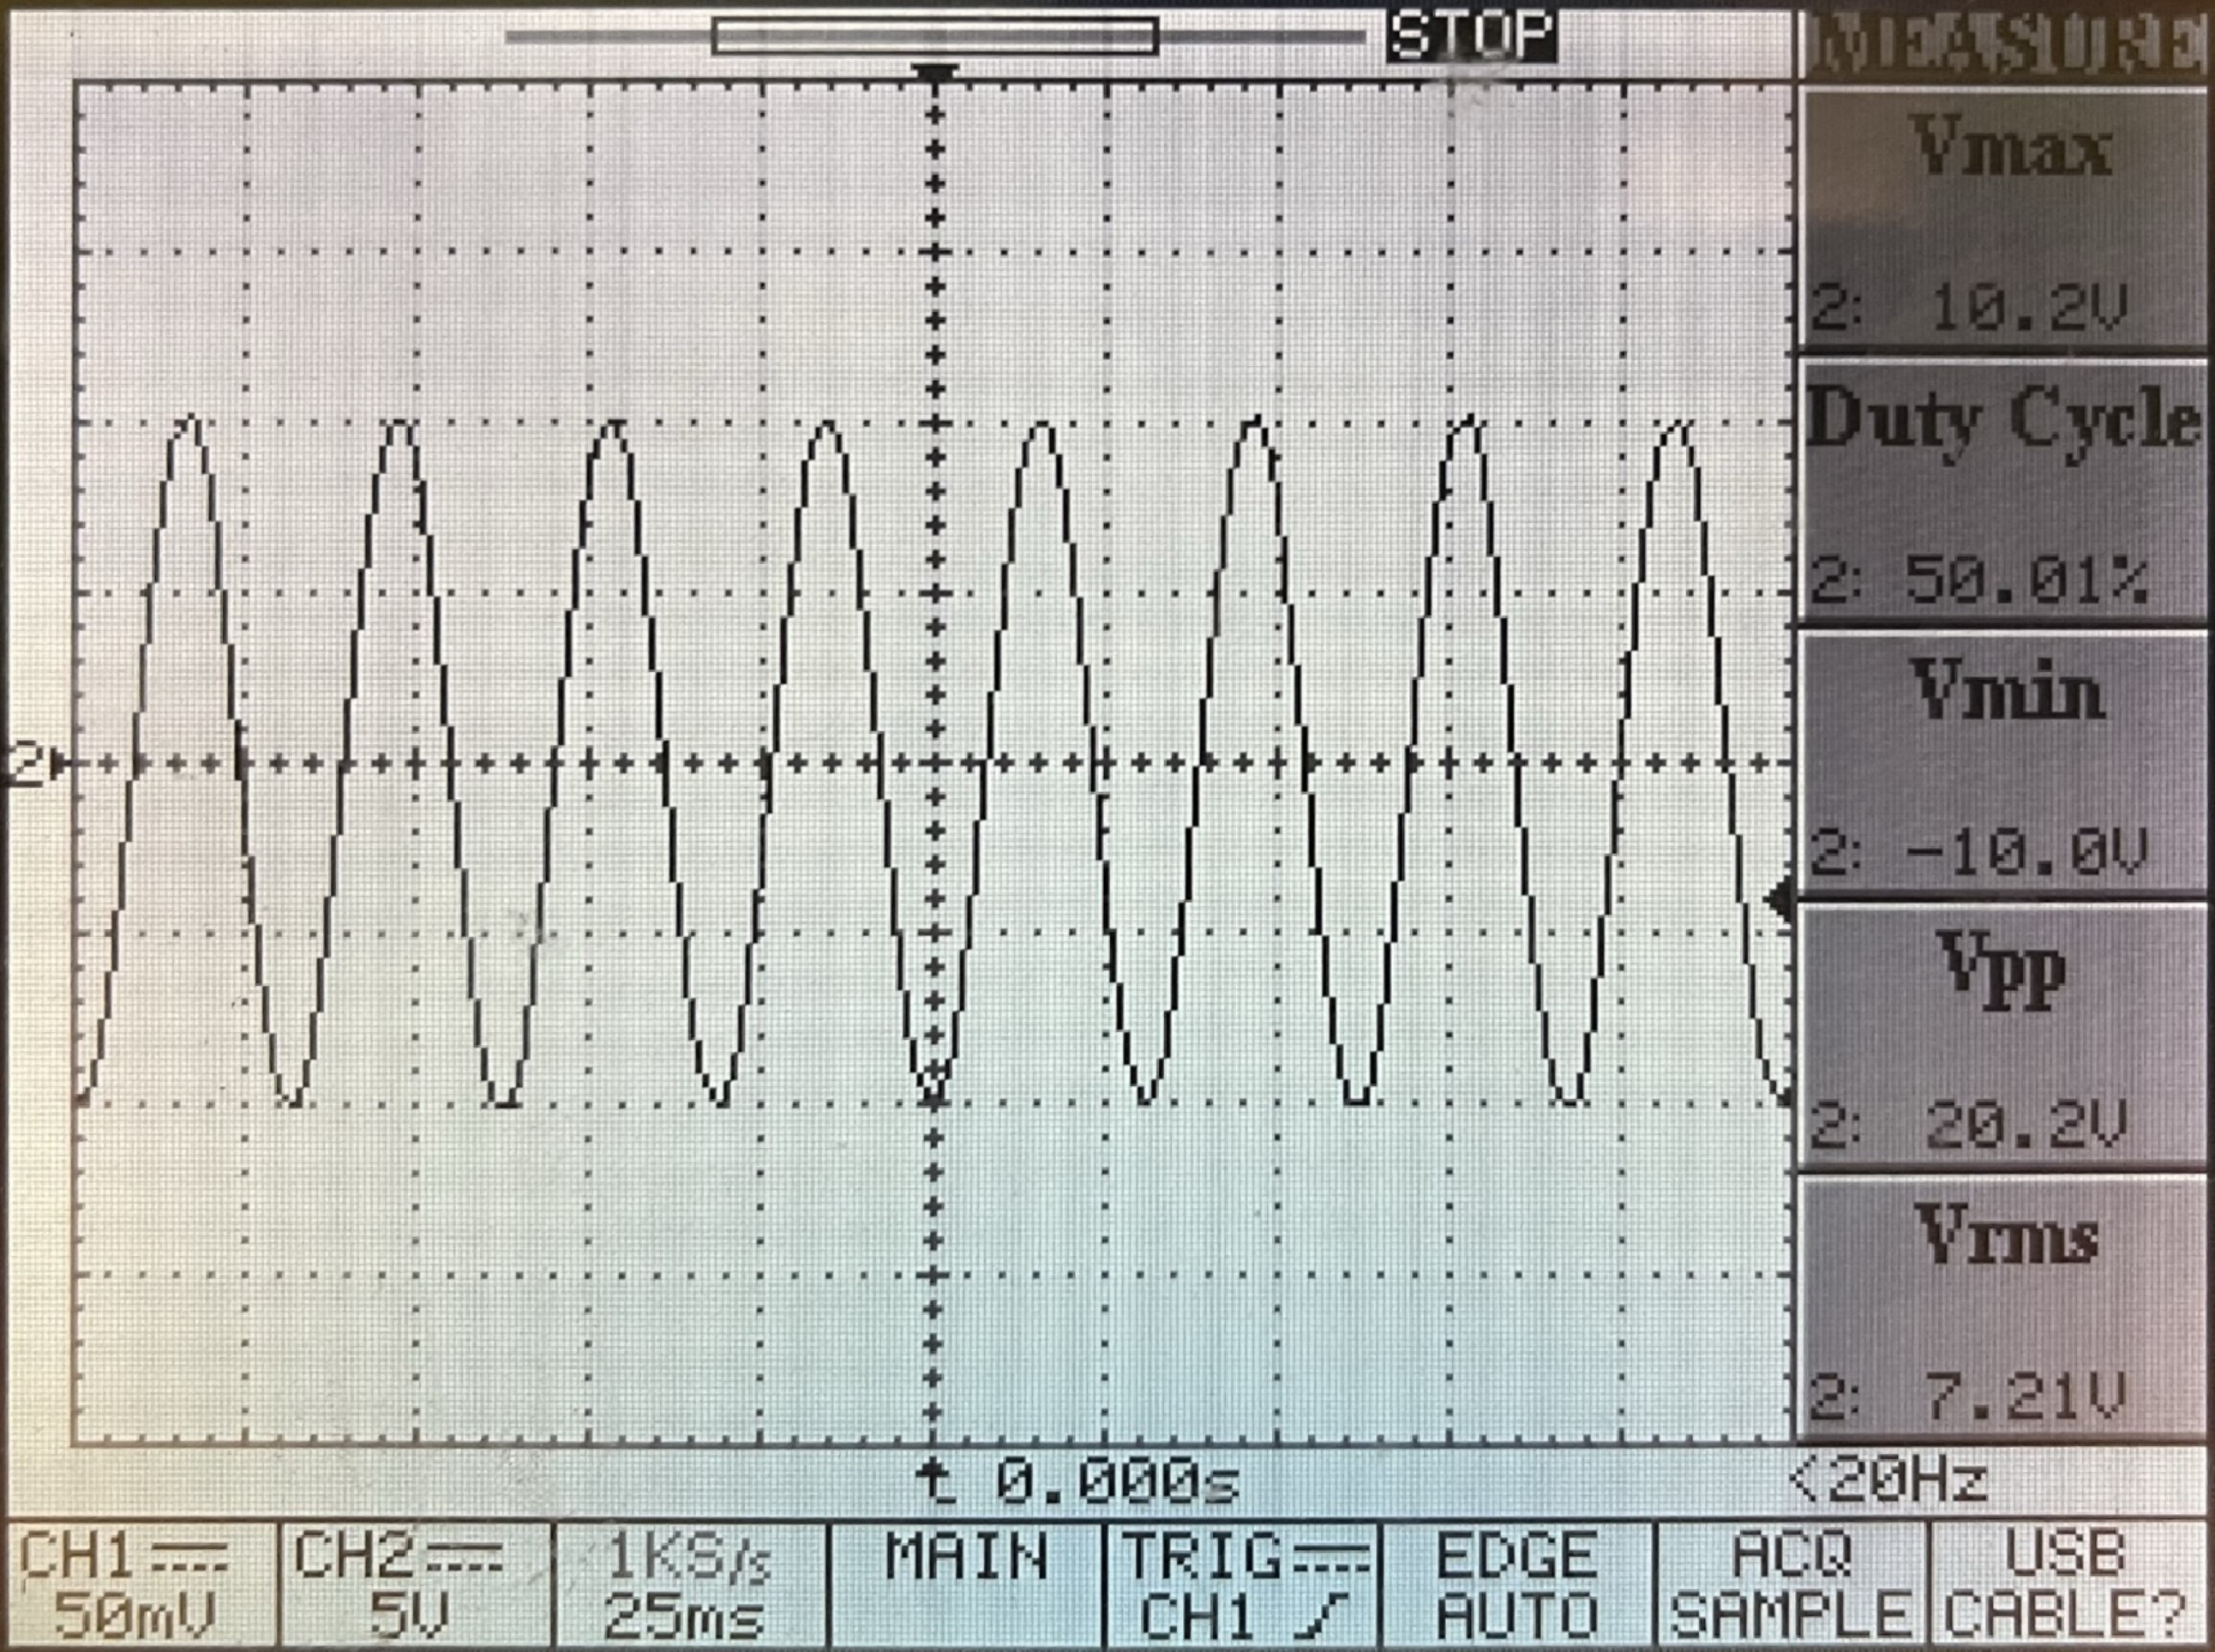
\includegraphics[width=0.6\textwidth]{Figures/flux_test.JPEG}
% 	\caption[Flux Linkage test, oscilloscope output @386rpm.]{Flux Linkage test, oscilloscope output @386rpm.}
% 	\label{fig:flux_measure_oscilloscope} %chktex 24
% \end{figure}

In the example image, the oscilloscope measured a peak voltage of $10.2$, while the rotor was spinning at $386rpm$, which is equivalent to $202rad/s$ electrical velocity. This results in a flux linkage of $0.050 Wb$. The same procedure was repeated at several speeds, and the results are shown in \Cref{fig:flux_linkage_rpm}. In this graph, two other lines are shown, they represent the flux linkage estimated using the torque and speed constant provided in the datasheet. Notice that the experimental data aligns well with the value derived from the voltage constant but it is very different from the value derived from the torque constant. This is probably due to different references and transformations being used, but as there isn't much information available on the datasheet, the measured value is assumed to be the correct one.

% \begin{figure}[!htb]
% 	\centering
% 	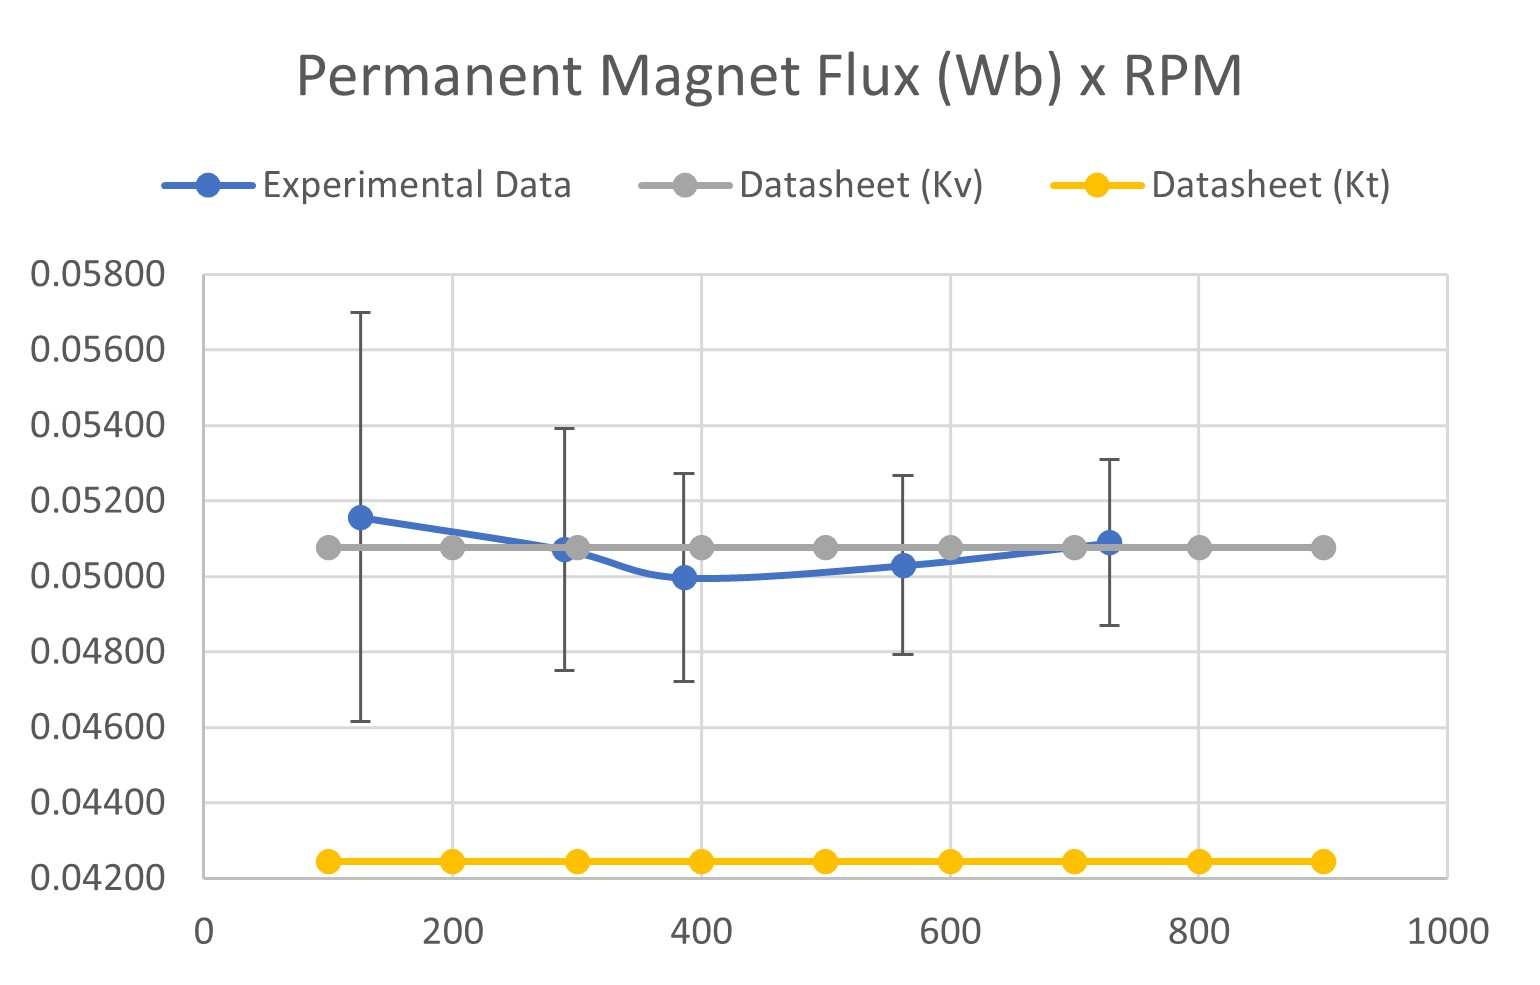
\includegraphics[width=0.5\textwidth]{Figures/flux_linkage_graph.jpg}
% 	\caption[Flux Linkage as a function of RPM.]{Flux Linkage as a function of RPM.}
% 	\label{fig:flux_linkage_rpm} %chktex 24
% \end{figure}
\begin{figure}[!htb]
    \begin{subfigmatrix}{2}
      \subfigure[Motor terminal voltage with rotor @386rpm]{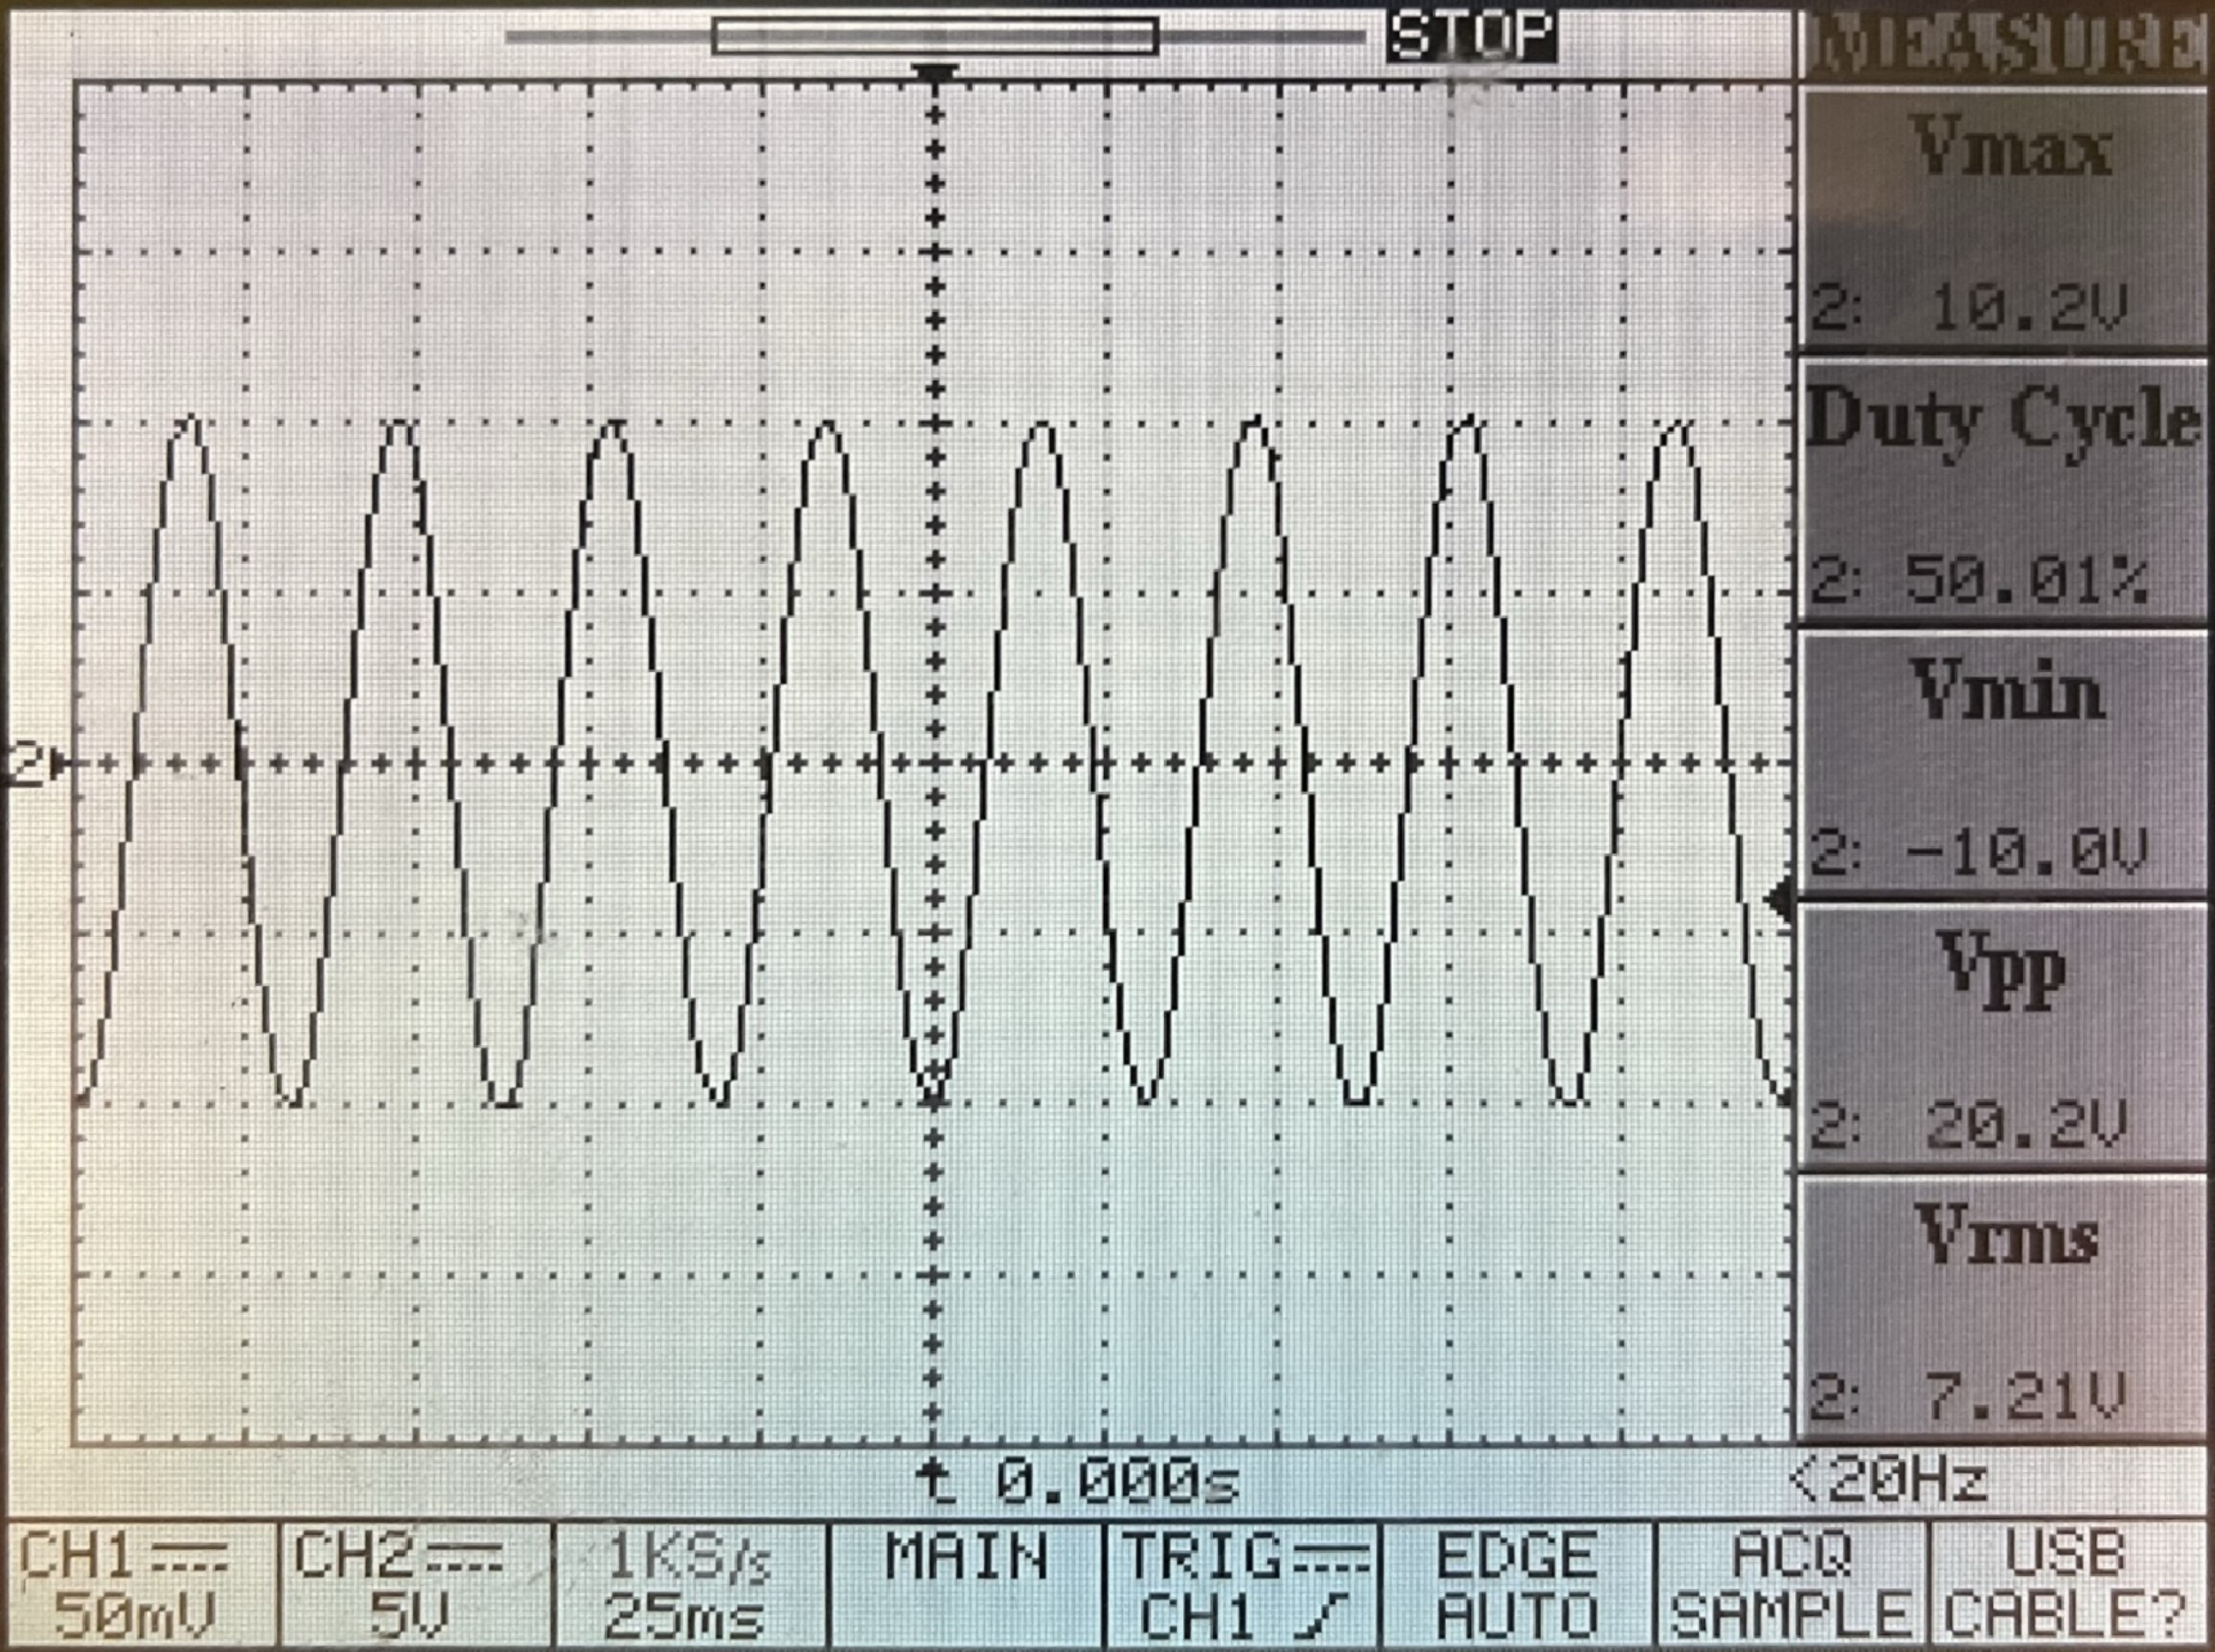
\includegraphics[width=0.51\textwidth]{Figures/flux_test.JPEG}\label{fig:flux_measure_oscilloscope}}
      \subfigure[Flux Linkage as a function of RPM.]{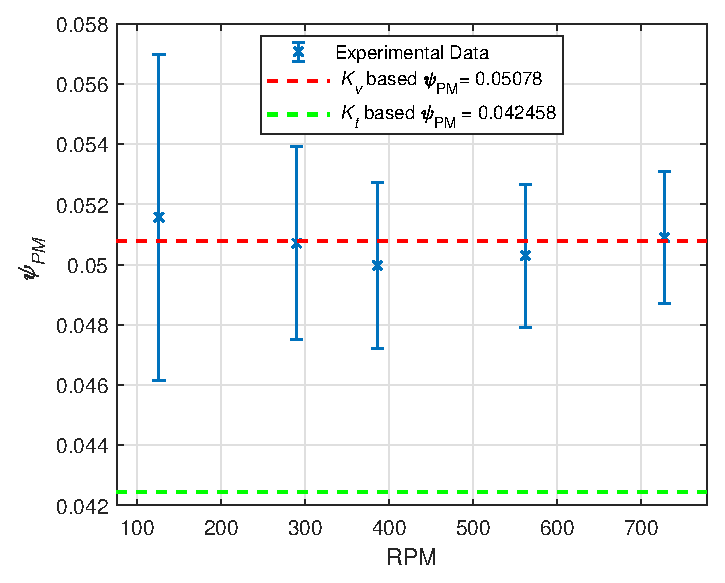
\includegraphics[width=0.45\textwidth]{Figures/Flux_test.eps}\label{fig:flux_linkage_rpm}}
    \end{subfigmatrix}
    \caption{Flux Linkage characterization.}
    \label{fig:flux_linkage_characterization}%chktex 24
\end{figure}

% %%%%%%%%%%%%%%%%%%%%%%%%%%%%%%%%%%%%%%%%%%%%%%%%%%%%%%%%%%%%%%%%%%%%%%%%%%%%%%%%%%%%%%%%%%%%%%%%%%%%%%%%%%%%%%%%%%%%%%%%%%%%%%%%%%%%%%%
% %%%%%%%%%%%%%%%%%%%%%%%%%%%%%%%%%%%%%%%%%%%%%%%%%%%%%%%%%%%%%%%%%%%%%%%%%%%%%%%%%%%%%%%%%%%%%%%%%%%%%%%%%%%%%%%%%%%%%%%%%%%%%%%%%%%%%%%
\subsection{Windings direct and quadrature inductances}
\label{sec:inductance}

To achieve better accuracy, two different methods will be proposed, one using the inverter, and the other only using a DC power supply.
\subsubsection{Method 1}
\label{sec:inductance_method1}

\begin{figure}[!htb]
	\centering
	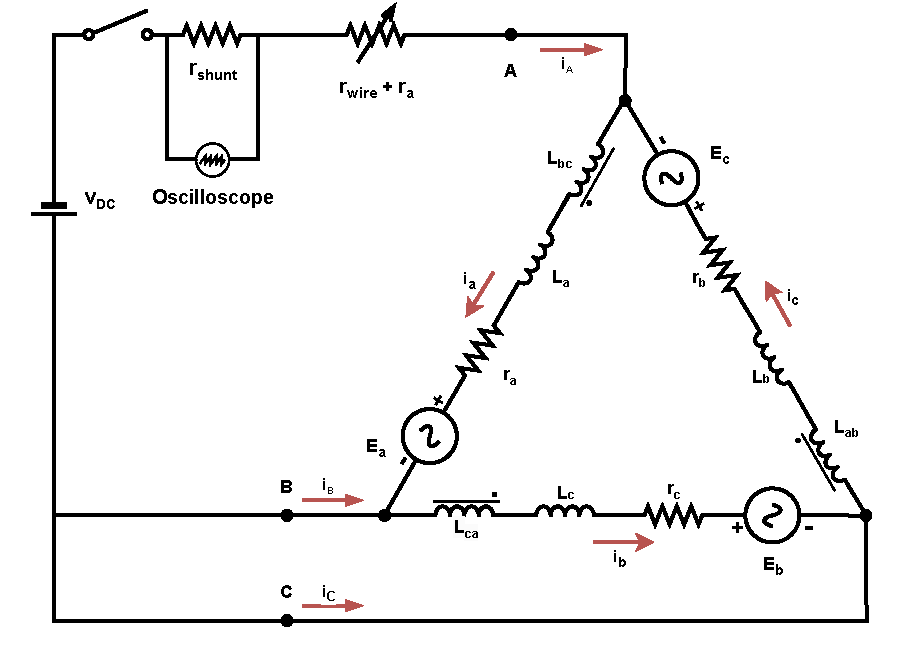
\includegraphics[width=0.6\textwidth]{Figures/Ld_measure.pdf}
	\caption[Inductance measurement setup schematic.]{Inductance measurement setup schematic.}
	\label{fig:Ld_measure_schematic} %chktex 24
\end{figure}

The simpler method, which does not use the inverter, works by measuring the current throughout a voltage step and measuring the time constant of the system. To measure the current, a shunt resistor is used coupled with the same oscilloscope from the previous section (\textit{Promax OD-571}). To achieve a variable current, a variable resistor was used in series with the shunt, as shown in \Cref{fig:Ld_measure_schematic}. The system resistance was measured with the micro ohmmeter from the previous section (\textit{UNI-T UT620A Micro-ohmmeter}), including wire and switch resistance. The experiment setup is shown in \Cref{fig:induc_setup}.
% \begin{figure}[!htb]
%     \begin{subfigmatrix}{2}
%       \subfigure[Schematic]{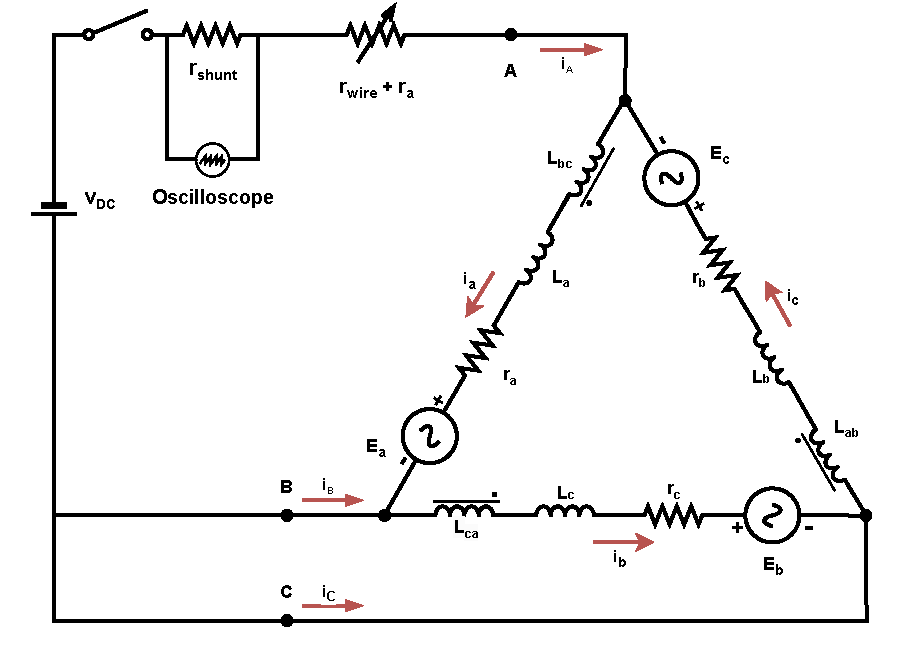
\includegraphics[width=0.49\linewidth]{Figures/Ld_measure.pdf}\label{fig:Ld_measure_schematic}}
%       \subfigure[Actual setup]{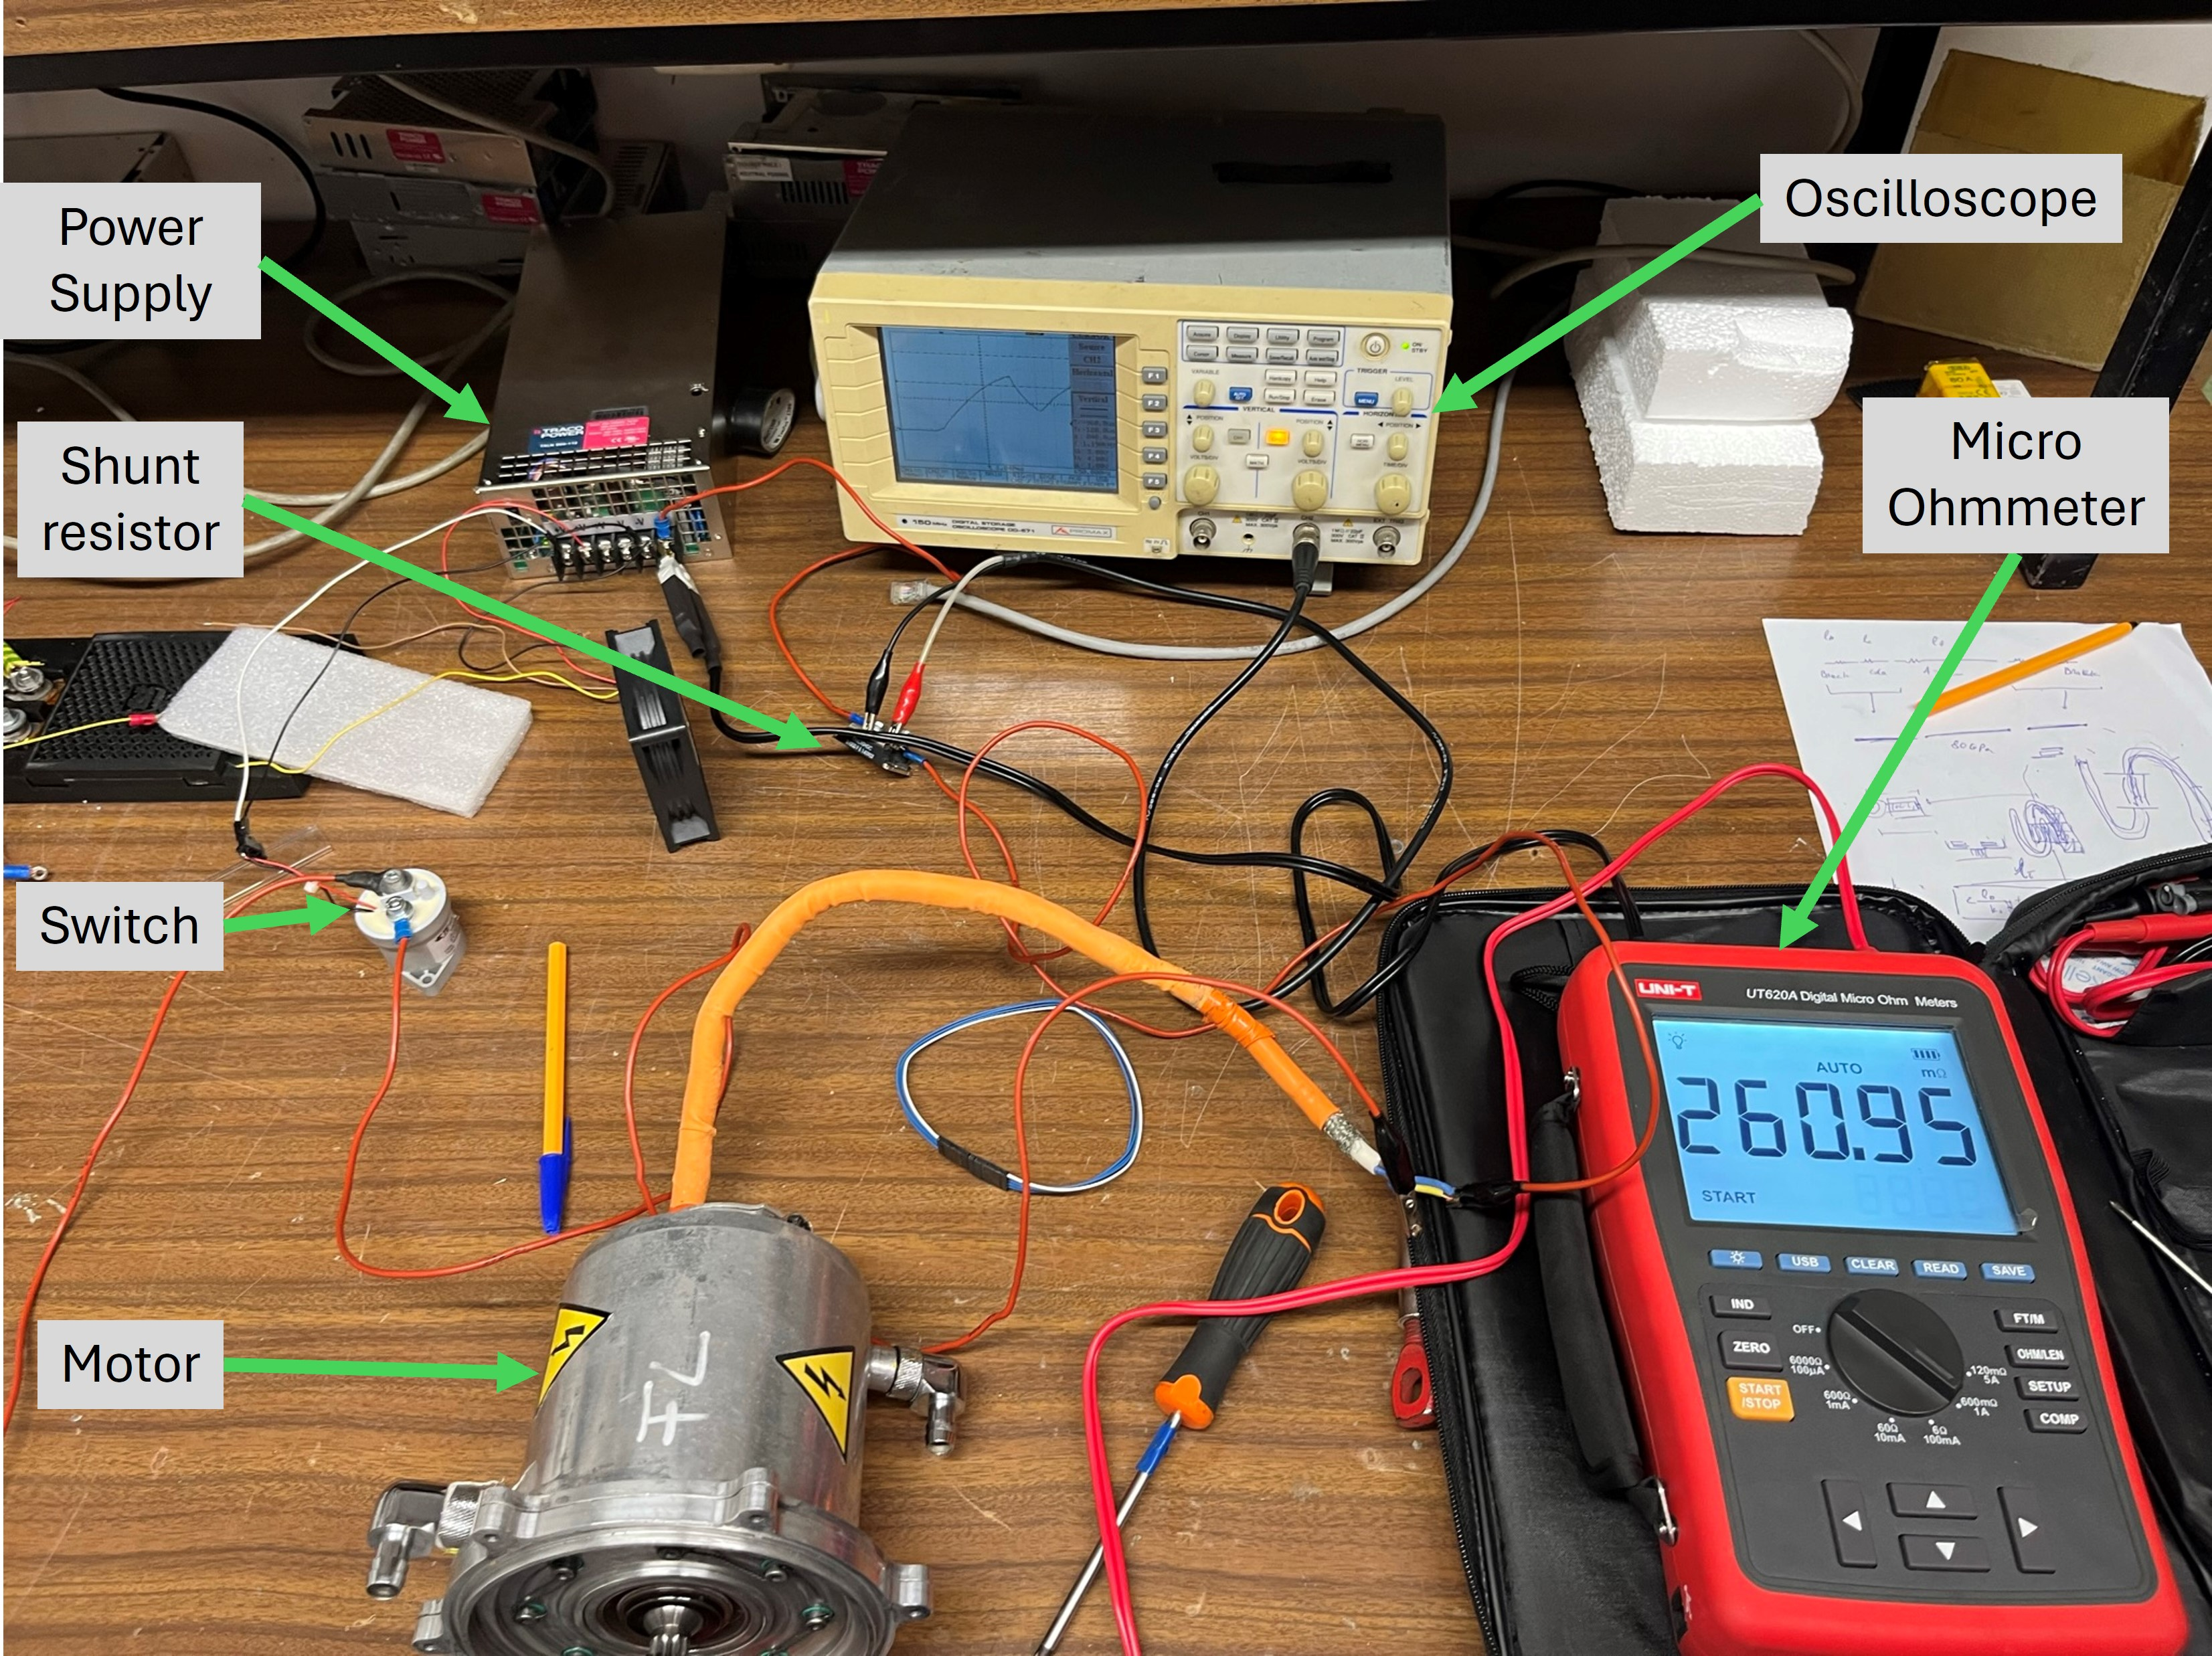
\includegraphics[width=0.49\linewidth]{Figures/induc_test.JPEG}\label{fig:induc_setup}}
%     \end{subfigmatrix}
%     \caption{Inductance measurement setup.}
%     \label{fig:aircrafts}%chktex 24
% \end{figure}


\begin{figure}[!htb]
	\centering
	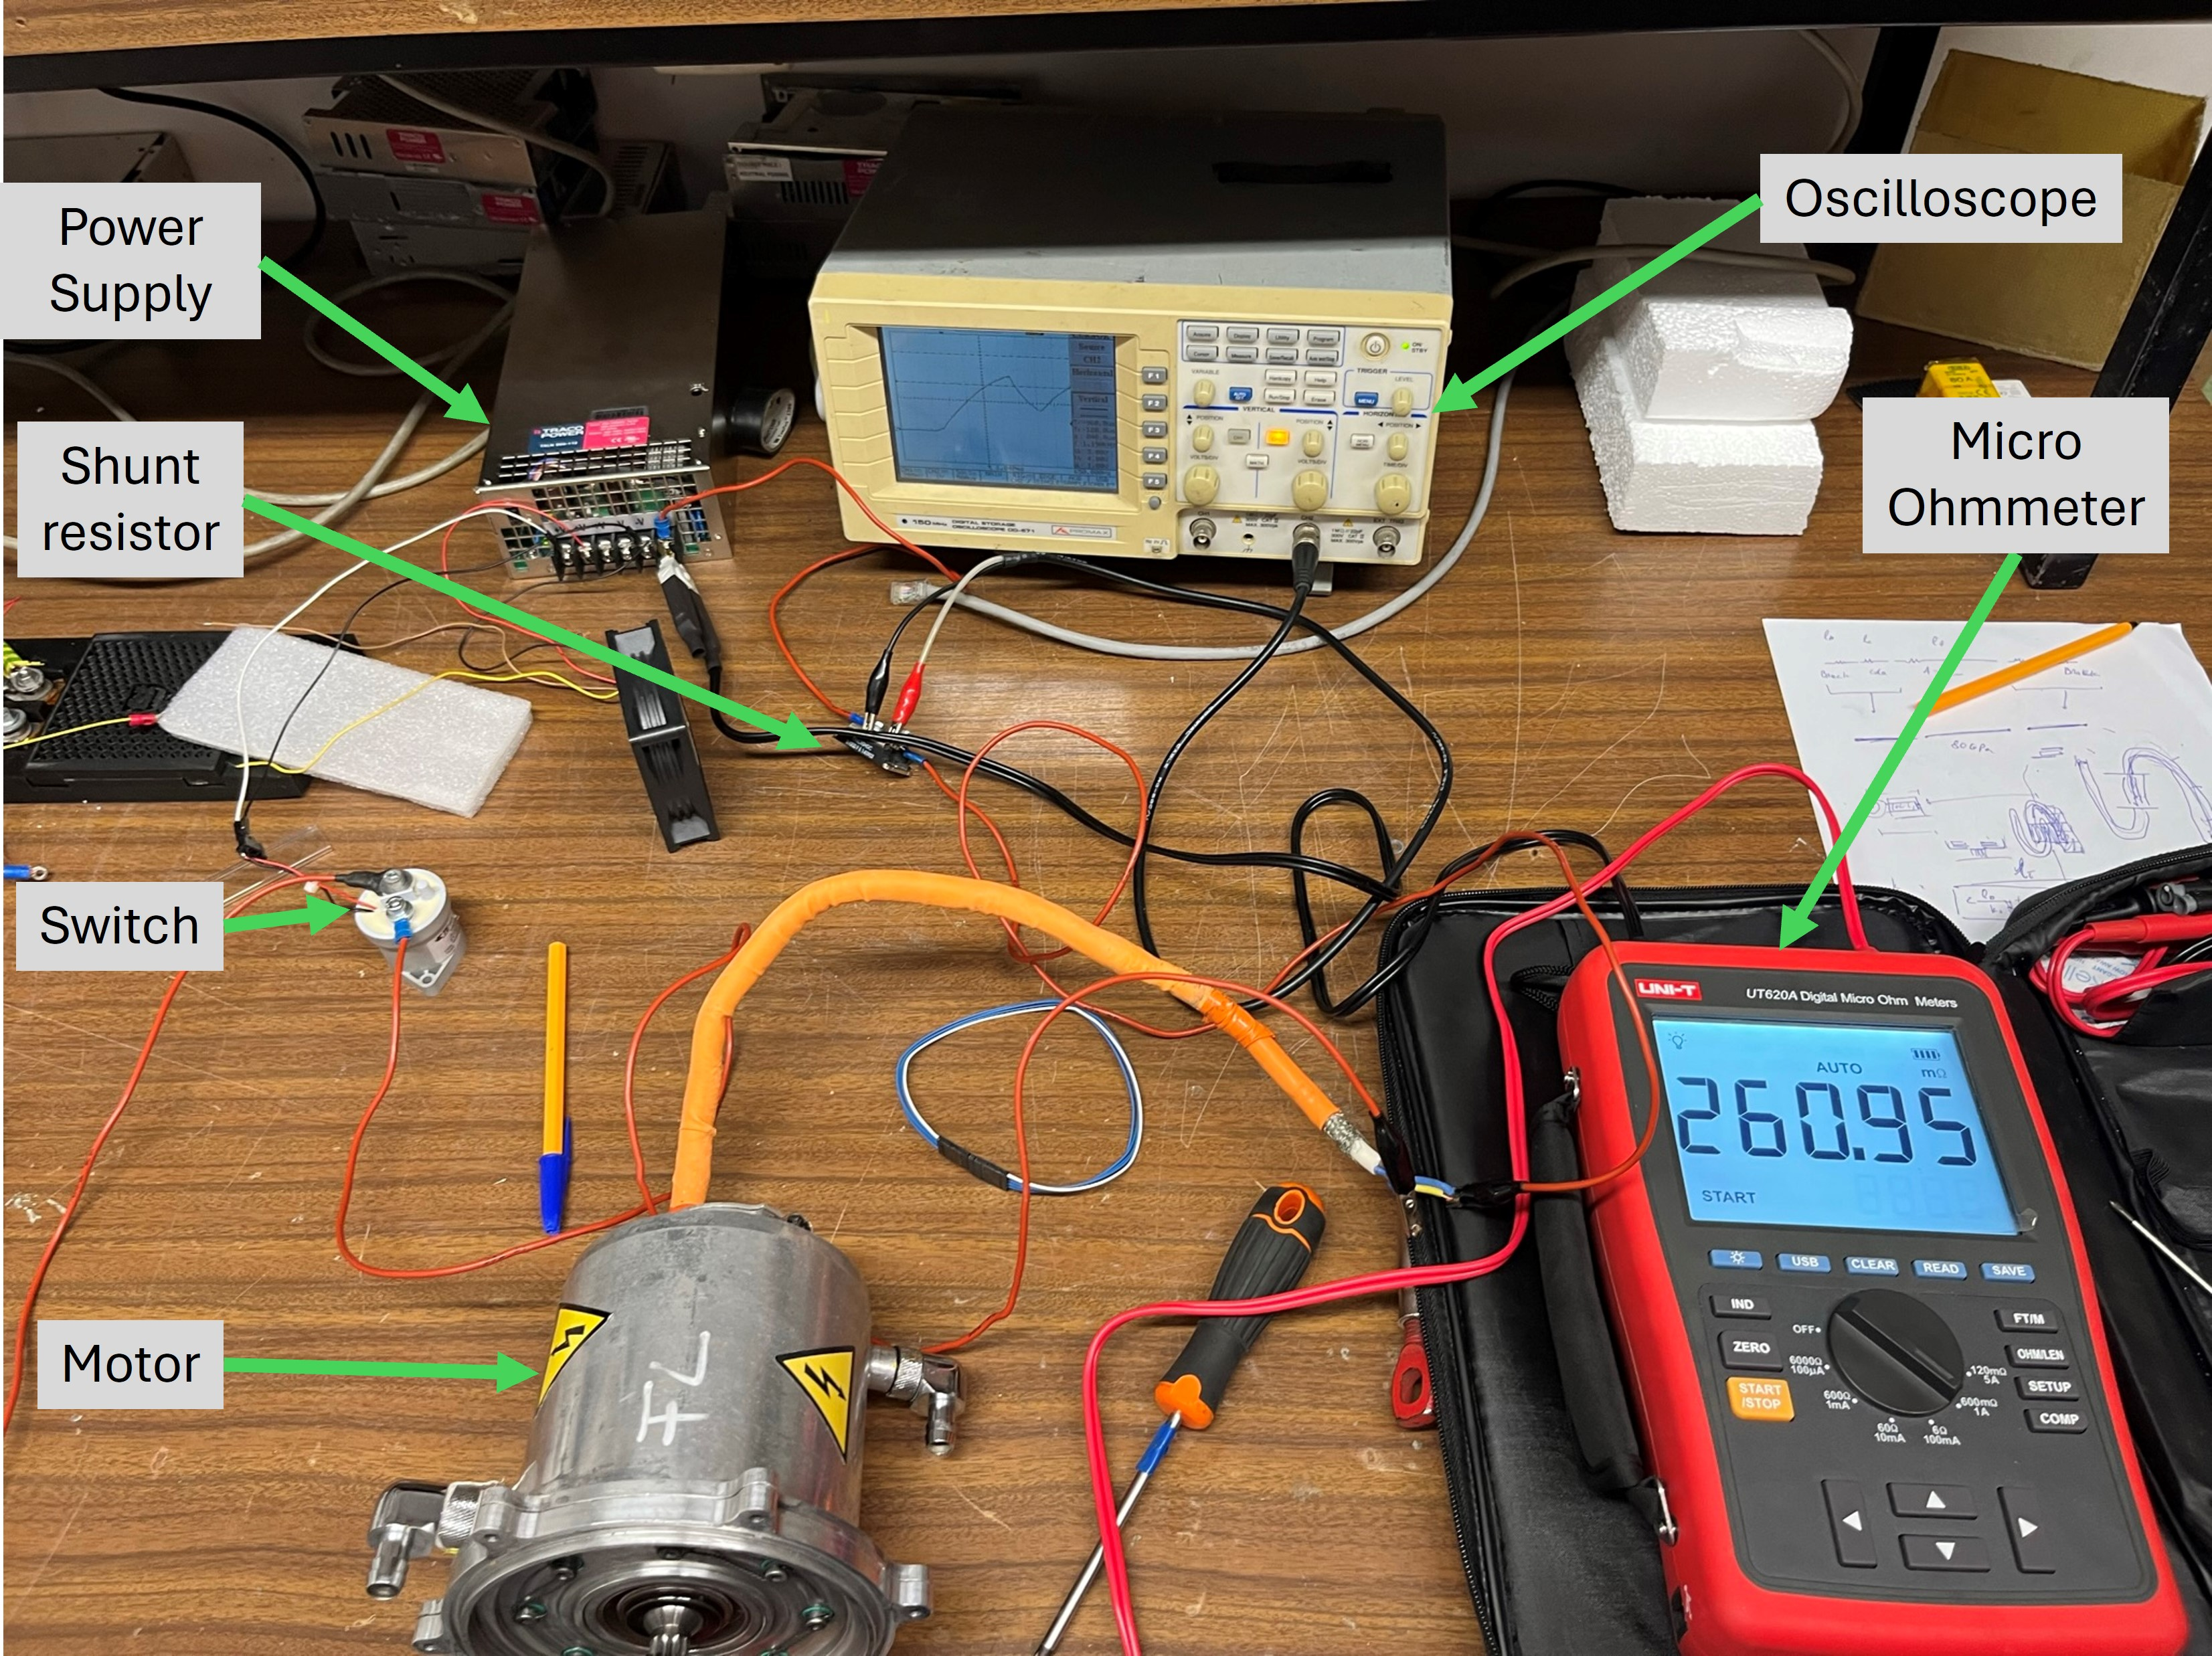
\includegraphics[width=0.6\textwidth]{Figures/induc_test.jpg}
	\caption[Inductance measurement setup.]{Inductance measurement setup.}
	\label{fig:induc_setup} %chktex 24
\end{figure}

\subsubsubsection{Direct Axis}
The direct axis measurement starts with the resistance measurement of the entire setup, motor, wires, switch, and shunt. Then, a quick voltage pulse is applied to align the rotor with the magnetic field, which in this setup is equivalent to the voltage vector $V_6$. In the aligned condition, the current through phase b ($i_b$) is zero, and $i_a = -i_c$. After the rotor is aligned, a new pulse is applied, now for the actual measurement as exemplified in \Cref{fig:inductance_oscilloscope}. The time constant can be retrieved using the basic equation for an RL circuit applied to the shunt resistor (\Cref{eq:rl_circuit,eq:tau}).

\begin{subequations}
	\begin{equation}
		u(t) = i_A r_{shunt}(1-e^{\frac{-t}{\tau}})
		\label{eq:rl_circuit}
	\end{equation}
	\begin{equation}
		\tau = \frac{0.5L_d}{\frac{r}{2}+r_{wire} + r_a + r_{shunt}}
		\label{eq:tau}
	\end{equation}
\end{subequations}
In \Cref{eq:rl_circuit} $u(t)$ represents the measured voltage on the shunt resistor, $V_{DC}$ is the power supply voltage, $\tau$ is the system time constant, $r_a$ is the variable resistance to adjust the current,$r_{shunt}$ is the shunt resistance, and $r_{wire}$ is the sum of the wire resistances with the switch resistance. 
% To simplify the measurements, instead of calculating the first term $i_A r_{shunt}$, it was replaced by the voltage that which the oscilloscope settled.

\begin{figure}[!htb]
	\centering
	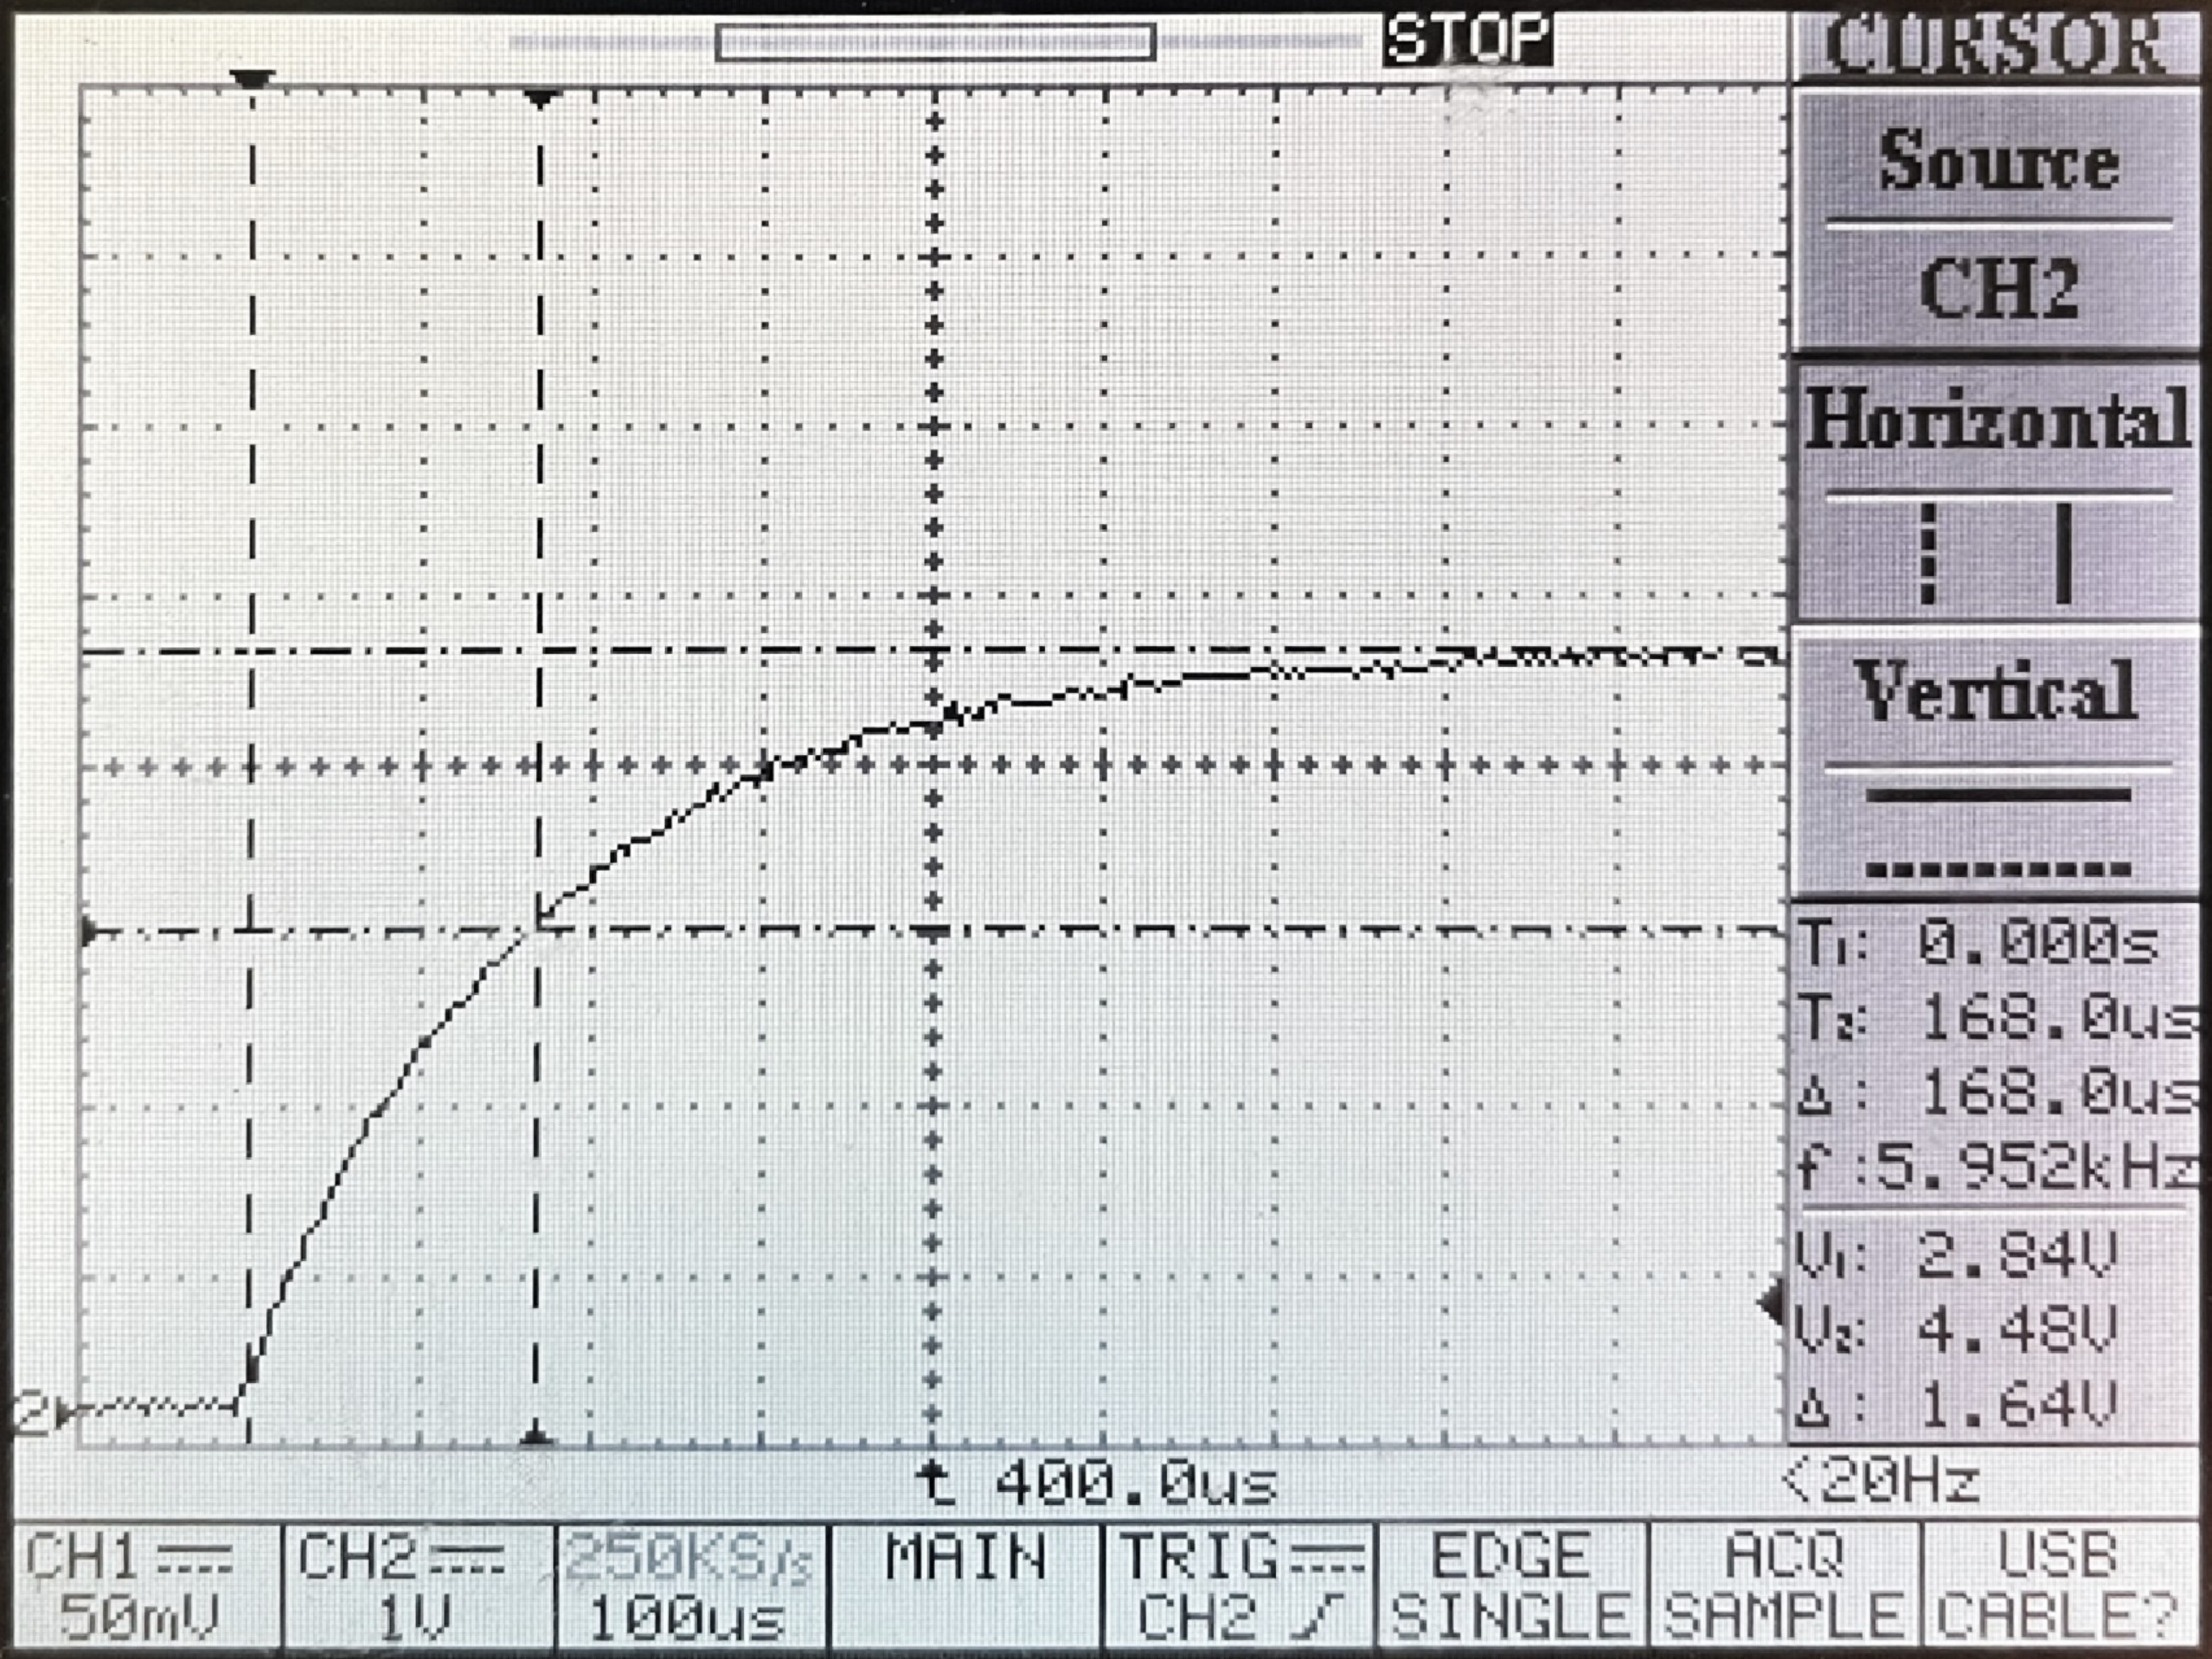
\includegraphics[width=0.5\textwidth]{Figures/induc_oscilloscope.JPEG}
	\caption[Example of the voltage step response used for the inductance characterization.]{Example of the voltage step response used for the inductance characterization.}
	\label{fig:inductance_oscilloscope} %chktex 24
\end{figure}

With the curve plotted on the oscilloscope, the time constant was measured by evaluating how long it took for the voltage to reach $0.632 i_A r_{shunt}$. Then, with the time constant and the system resistance, the inductance was calculated. Note that this inductance was measured for a phase current of half the line current, resulting in a direct axis current of $i_d = \frac{i_A}{\sqrt{3}}$.

The inductance variation with current is not symmetrical in the current axis, as the permanent magnet offsets the magnetic curve, causing saturation with very small positive currents in the direct axis. Although simple, this method has the drawback of not measuring the variation of inductance in the field weakening operating range, only on the field intensifying range that is not often used. To measure in the field weakening range it is necessary to lock the rotor after the initial pulse, and then invert the power supply polarity.

\begin{figure}[!htb]
	\centering
	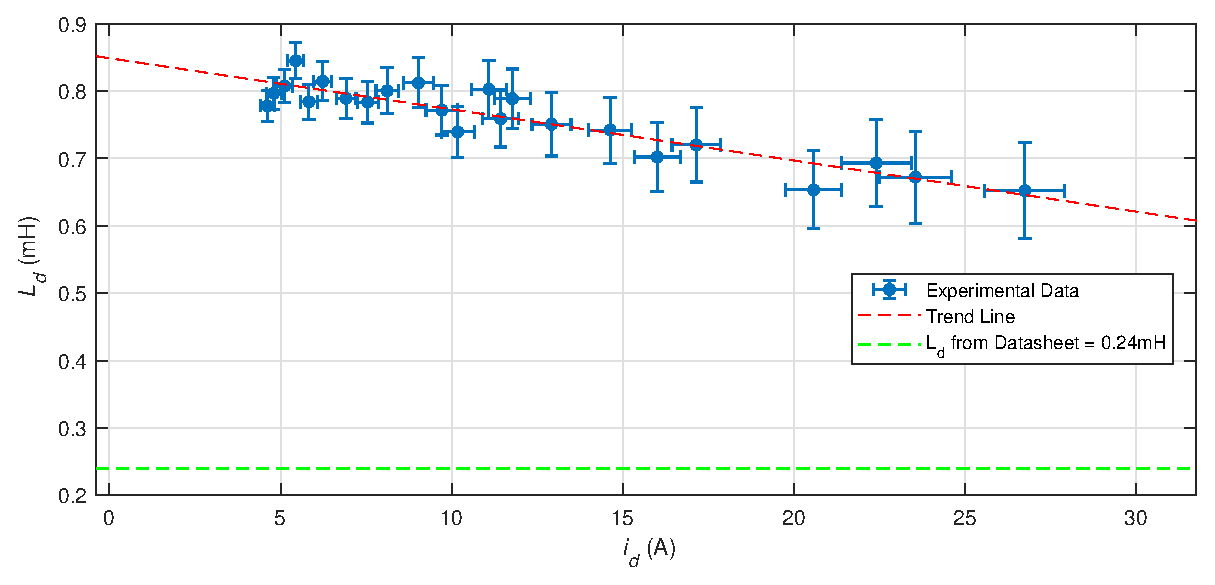
\includegraphics[width=1\textwidth]{Figures/Ld_id.eps}
	\caption[$L_d$ in function of $i_d$.]{$L_d$ in function of $i_d$.}
	\label{fig:ld_graph} %chktex 24
\end{figure}

The test results are shown in \Cref{fig:ld_graph}, and as with the flux linkage, there is a great difference between the measured data and the value from the datasheet. The saturation effects are clear and start with very little current, as predicted.




\subsubsubsection{Quadrature Axis}
The quadrature axis measurement is very similar to the direct axis, with only two differences. The first change is on the alignment pulse, instead of shorting the B and C terminals and applying the pulse from A to BC as done for the direct inductance measurement, the pulse is only applied from B to C as shown in \Cref{fig:quad_induc_setup_prep}. This will align the rotor with the phase b axis allowing it to be locked in a position electrically orthogonal to the resultant voltage of a pulse from A to BC\@. That is the second difference, after the alignment an external tool is necessary to lock the rotor in place. The rest of the procedure is the same as the direct axis measurement.

\begin{figure}[!htb]
	\centering
	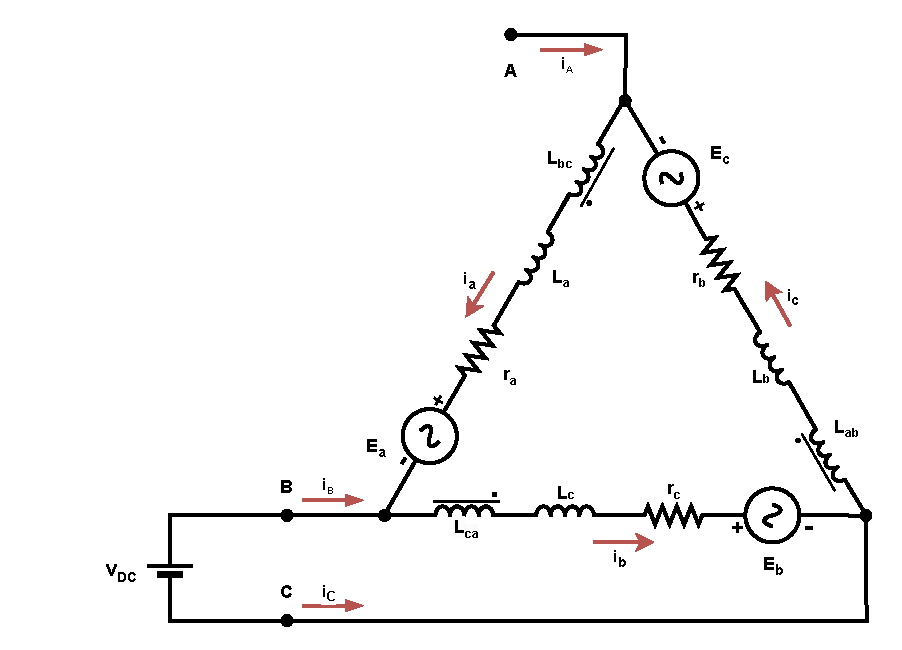
\includegraphics[width=0.7\textwidth]{Figures/Lq_measure_prep.pdf}
	\caption[Quadrature Inductance measurement alignment pulse setup.]{Quadrature Inductance measurement alignment pulse setup.}
	\label{fig:quad_induc_setup_prep} %chktex 24
\end{figure}

The results of the quadrature inductance are shown in \Cref{fig:lq_graph}. It is important to note that as there isn't a reminiscent magnetic flux in the quadrature axis, the variation of the inductance with current is symmetrical in the current axis, and only shows signs of saturation at high currents.

\begin{figure}[!htb]
	\centering
	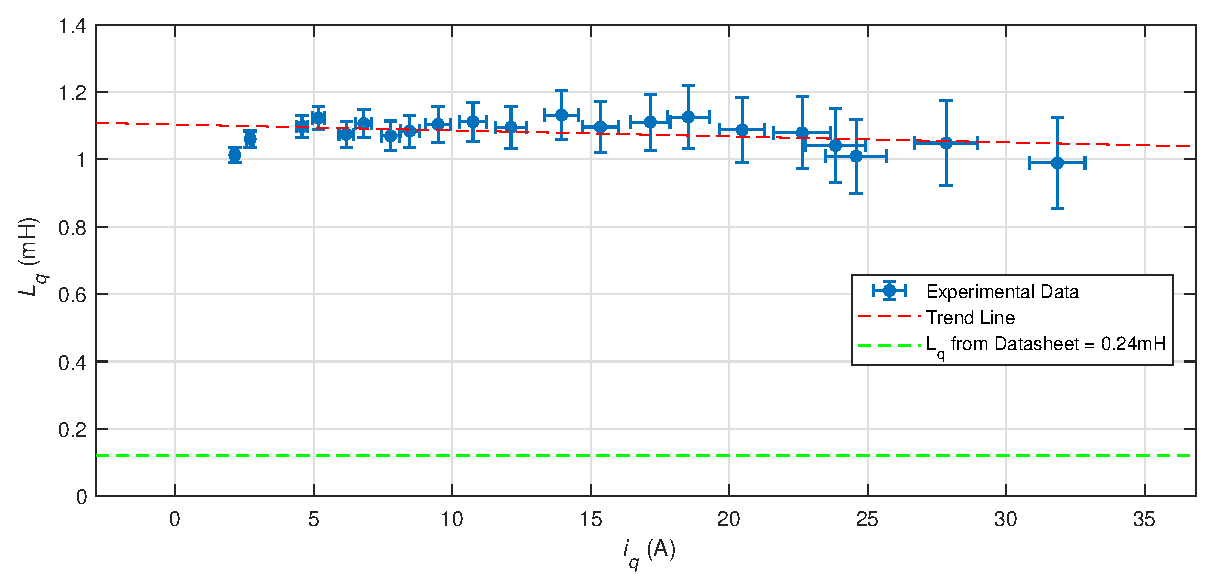
\includegraphics[width=1\textwidth]{Figures/Lq_iq.eps}
	\caption[$L_q$ in function of $i_q$.]{$L_q$ in function of $i_q$.}
	\label{fig:lq_graph} %chktex 24
\end{figure}

\subsubsection{Method 2}

The second method for inductance characterization is according to~\citet{Stumberger:saturation_model:2003}. It uses a \gls{vsi} coupled with a control algorithm to keep the current in one of the axis constant, and then do a voltage step in the other axis. This measurement also needs to be done in a locked rotor position, but it has the advantage of characterizing the cross-magnetization effect. The rotor needs to be locked to allow the simplification shown in \Cref{eq:motor_with_no_omega}, resulting in \Cref{eq:inductance_voltage_step}.

\begin{subequations}
	\begin{equation}
		u_d = ri_d(t) + \frac{d\psi_d (t)}{dt} - \psi_q \cancelto{0}{\omega_e}
	\end{equation}
	\begin{equation}
		u_q = ri_q(t) + \frac{d\psi_q (t)}{dt} + \left(\psi_d + \psi_{PM}\right) \cancelto{0}{\omega_e}
	\end{equation}
	\label{eq:motor_with_no_omega}
\end{subequations}


\begin{subequations}
	\begin{equation}
		\frac{d\psi_d (t)}{dt} = u_d - ri_d(t)
	\end{equation}
	\begin{equation}
		\frac{d\psi_q (t)}{dt} = u_q - ri_q(t)
	\end{equation}
	\label{eq:inductance_voltage_step}
\end{subequations}

This method defines the flux linkage based on the integration of \Cref{eq:inductance_voltage_step}, and to measure the flux linkage variation in the quadrature axis, it performs a series of stepwise voltage changes in $u_q$ while maintaining the current $i_d$ constant (\Cref{fig:stepwise}). The integration of those curves will result in the quadrature flux linkage variation with $i_q$. These steps are repeated for several values of $i_d$, and for each of them, a flux linkage curve is created as shown in \Cref{fig:flux_linkage_curve}. Note that this figure was generated as a concatenation of two separate voltage steps, one positive and one negative, to simplify the process. This concatenation is the reason for the small misalignment in the flux linkage lines near the origin.

Instead of using the measured value for the phase resistance, its value is estimated by assuming the current is at a steady state at the end of the voltage pulse so that the flux linkage is stable and $u_x = ri_x$, this is done to reduce integration errors on the flux linkage and also to account for wires, connections, and \gls{mosfet} resistances.

\begin{figure}[!htb]
	\begin{subfigmatrix}{2}
		\subfigure[Voltage]{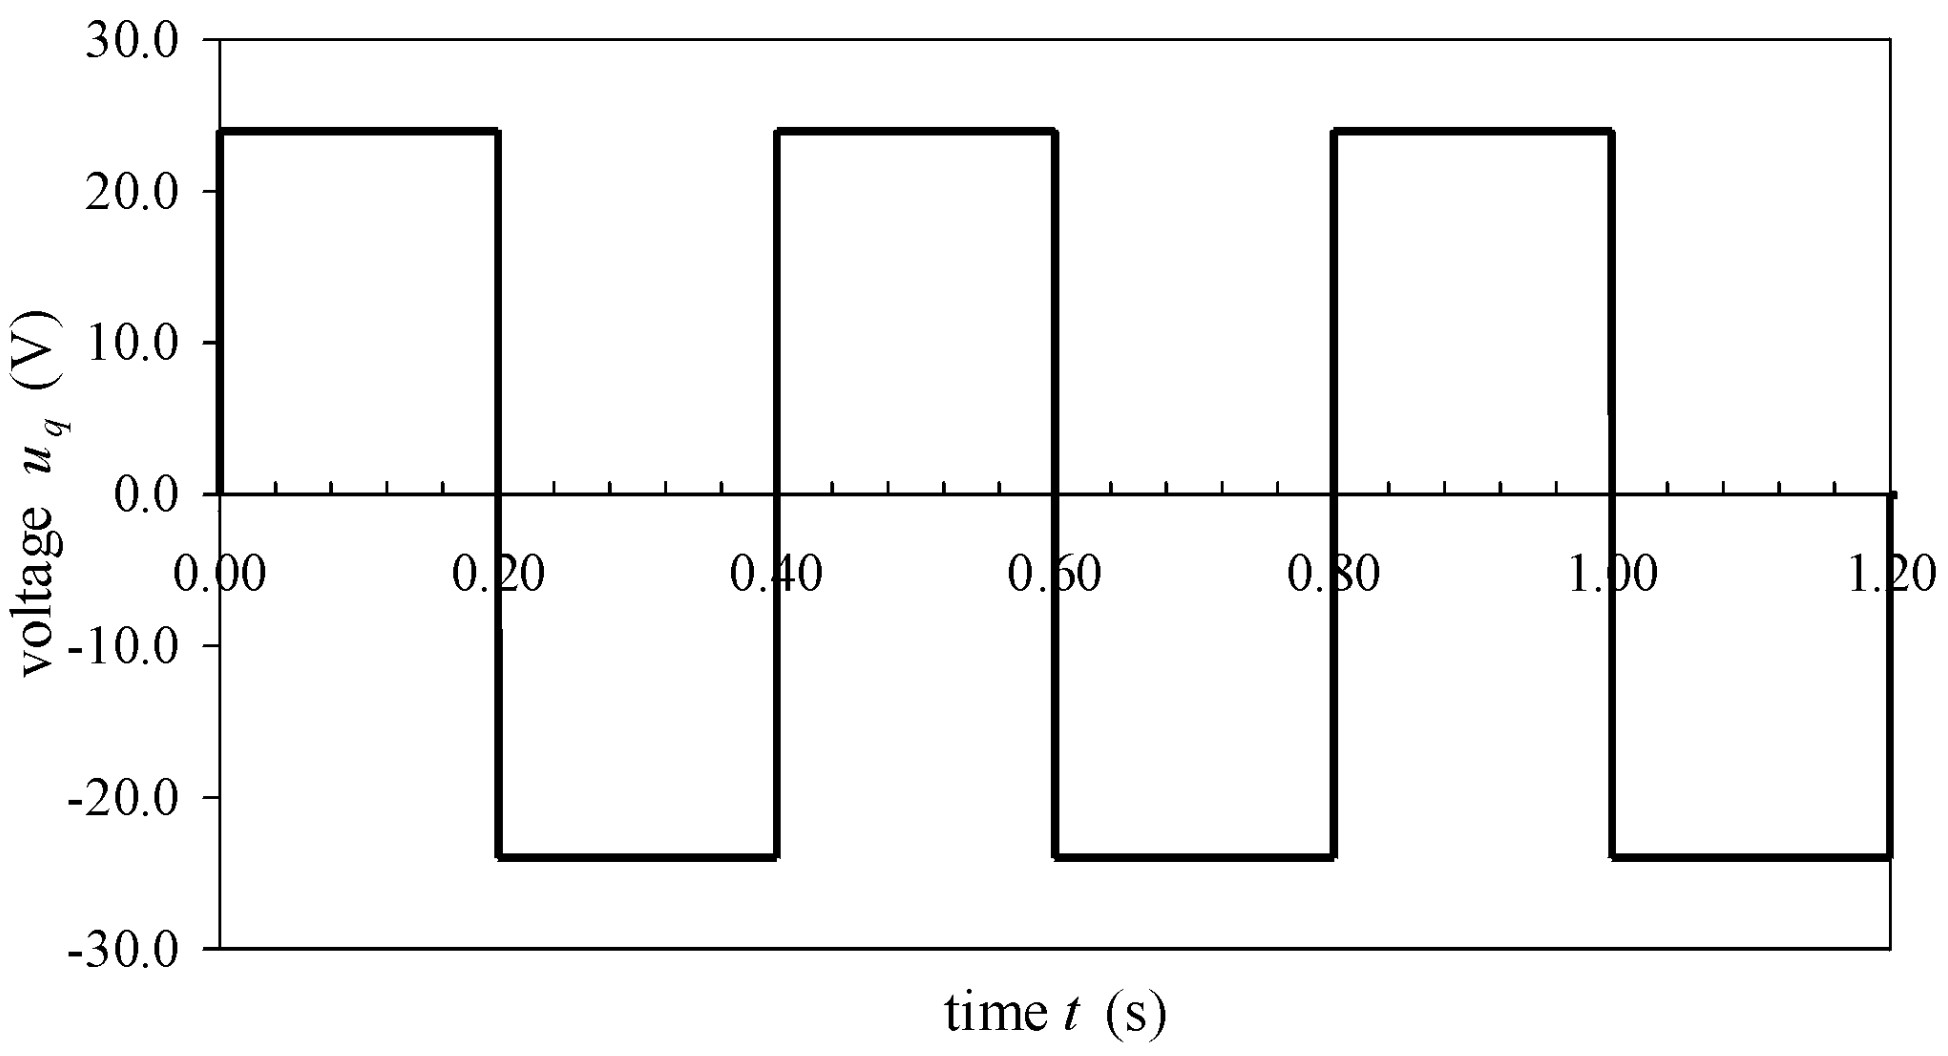
\includegraphics[width=0.49\linewidth]{Figures/stepwise_uq.jpg}\label{fig:stepwise_uq}}
		\subfigure[Currents]{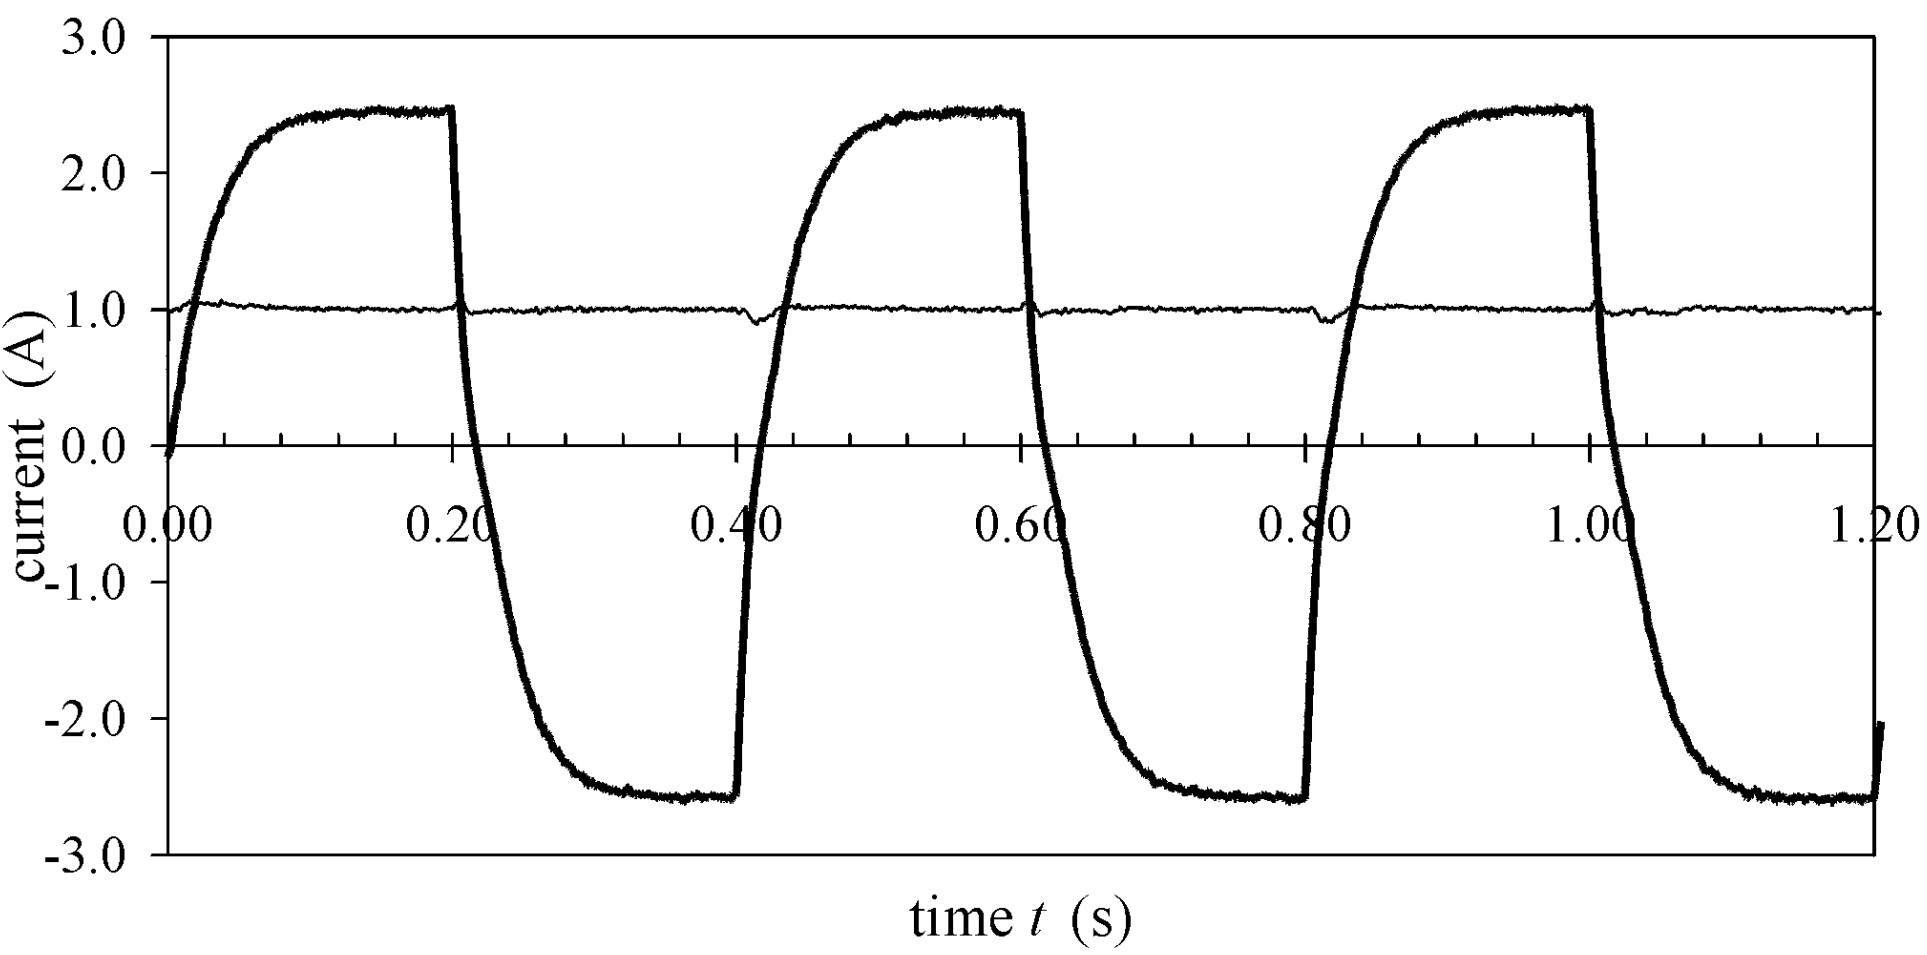
\includegraphics[width=0.49\linewidth]{Figures/stewise_currents_response.jpg}\label{fig:stepwise_currents}}
	\end{subfigmatrix}
	\caption{Identification voltage pulses - from~\citet{Stumberger:saturation_model:2003}.}
	\label{fig:stepwise}%chktex 24
\end{figure}
\begin{figure}[!htb]
	\centering
	\includegraphics[width=0.6\textwidth]{Figures/id-5__vq-30.eps}
	\caption[Quadrature Flux linkage @$i_d = -5$A.]{Quadrature Flux linkage @$i_d = -5$A.}
	\label{fig:flux_linkage_curve} %chktex 24
\end{figure}

The same procedure is used for measuring $\psi_d$, but this time the quadrature current is fixed and the direct voltage is changed in stepwise form. Although the original method is proposed to characterize cross-magnetization effects, the results shown in \Cref{fig:all_pulses} present little variation with currents on the perpendicular axis, thus to simplify the study they are approximated as independent. This approximation is used to reduce the dimensionality of the current reference table and to reduce the used space on the \gls{fpga}. To improve the efficiency of the process the quadrature flux linkage was not characterized for positive and negative currents, as the direct axis was, but only for negative currents. Due to the symmetry of the motor, the quadrature axis results were mirrored to create the flux values for positive and negative currents, as shown in \Cref{fig:all_pulses}.

\begin{figure}[!htb]
	\centering
	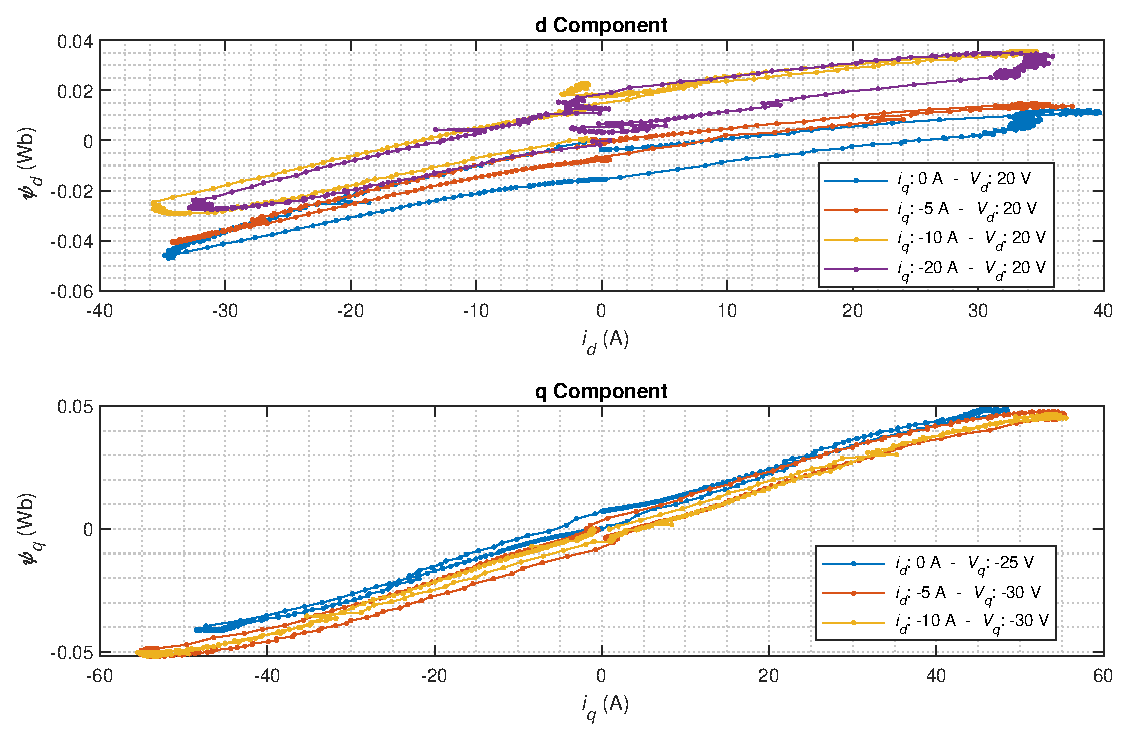
\includegraphics[width=1\textwidth]{Figures/all_pulses.eps}
	\caption[Flux linkage with different currents on a perpendicular axis.]{Flux linkage with different currents on a perpendicular axis.}
	\label{fig:all_pulses} %chktex 24
\end{figure}
%explain about the fit  and the derivative, reinforece that we decided to not account for crossmagnetization to simplify the computations and reduce the size of the lookup table
After the characterization of the fluxes, an exponential fit is done to the data as shown in \Cref{fig:inductances_method_2}. This fit is made disregarding cross magnetization effects, as explained before, and uses the format of \Cref{eq:flux_linkage_fit}. This allows analytical differentiation, resulting in \Cref{eq:flux_derivative_inductance}. This derivative is the inductance value for the given current on the respective axis.
%	\psi_x = ( a1*exp(-b1*x)+ a2*exp(-b2*x)) + c + c_up*((1)/(a4*exp(-b4*x)+1))+c_down*(1-((1)/(a3*exp(-b3*x)+1)))
\begin{equation}
	\psi_x = ( a_1 \cdot e^{-b_1 \cdot x}+ a_2 \cdot e^{-b_2 \cdot x}) + c_{down}\left(1-\left(\frac{1}{a_3 \cdot e^{-b_3 \cdot x}+1}\right)\right) + c_{up} \left(\frac{1}{a_4 \cdot e^{-b_4 \cdot x}+1}\right) + c
	\label{eq:flux_linkage_fit}
\end{equation}
% Here a repeated subscript represents the self-inductance, while multiple subscript identifiers represent mutual inductances due to crossmagnetization.

\begin{figure}[!htb]
	\centering
	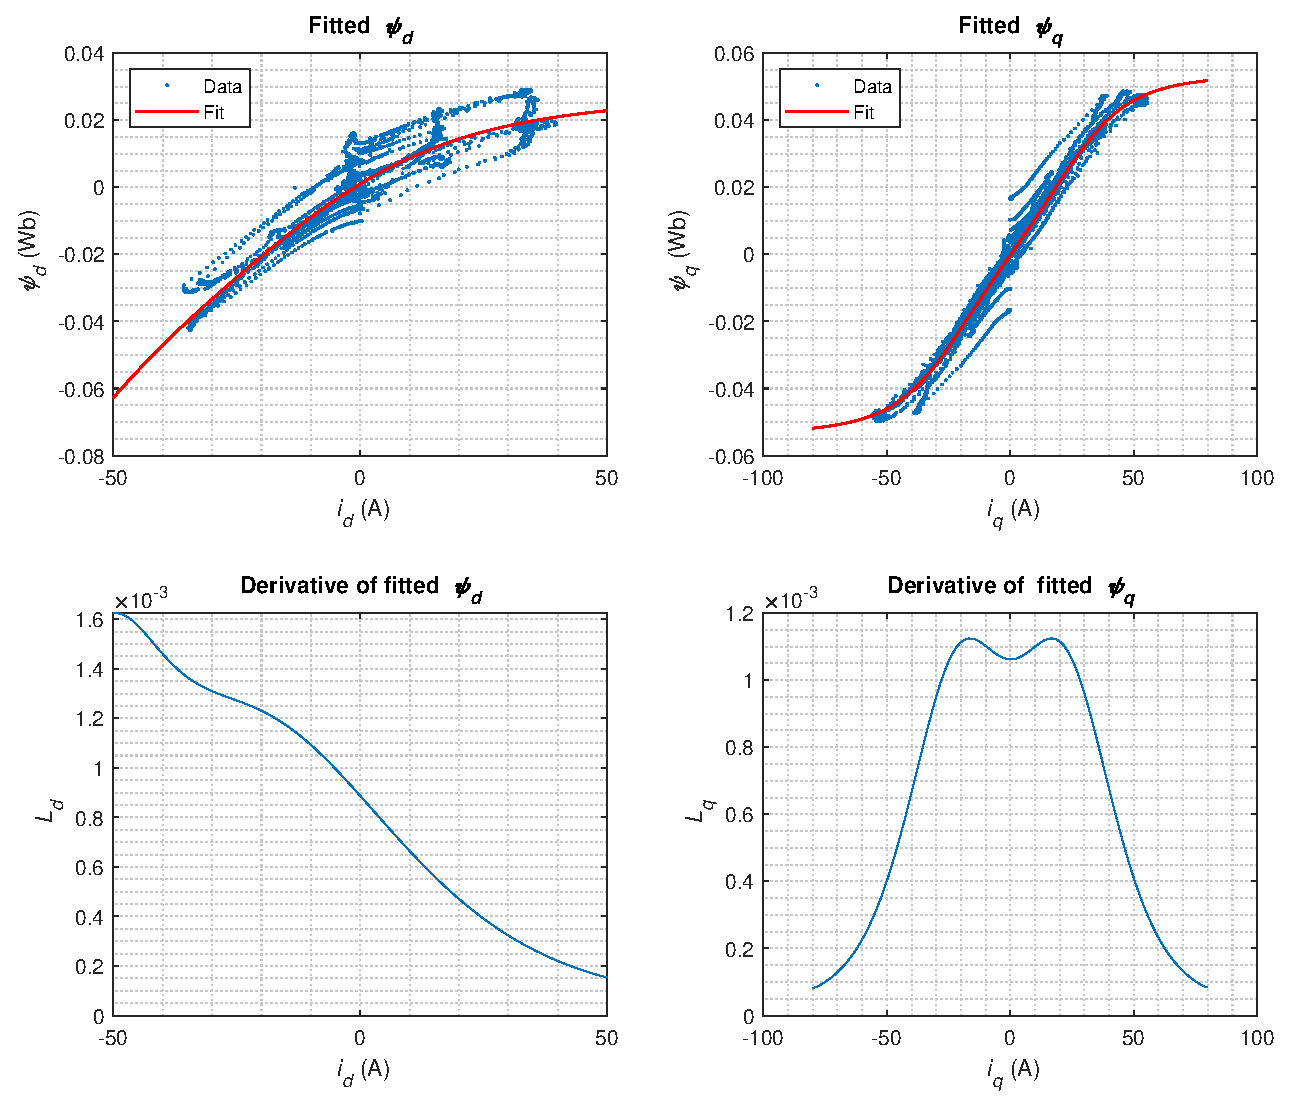
\includegraphics[width=1\textwidth]{Figures/Ldq.eps}
	\caption[Flux Linkage exponential fit.]{Flux Linkage exponential fit. The blue dots are the measured flux linkage, while the red line is the exponential fit (R-square 0.8879 for $\psi_d$ and 0.9681 for $\psi_q$). The bottom plots show the inductances as the derivative of the fit.}
	\label{fig:inductances_method_2} %chktex 24
\end{figure}
\begin{subequations}
		\noindent
		\begin{minipage}{.5\linewidth}
			\begin{equation}
				L_{d} = \frac{\partial \psi_d}{\partial i_d} \approx \frac{\Delta \psi_d}{\Delta i_d}
				% \at[\bigg]{i_q=\text{const.}}
			\end{equation}
		\end{minipage}%
		\begin{minipage}{.5\linewidth}
			\begin{equation}
				L_{q} = \frac{\partial \psi_q}{\partial i_q} \approx \frac{\Delta \psi_q}{\Delta i_q}
				% \at[\bigg]{i_d=\text{const.}}
			\end{equation}
		\end{minipage}%\\
		\label{eq:flux_derivative_inductance}
	\end{subequations}
% \begin{subequations}
% 	\noindent
% 	\begin{minipage}{.5\linewidth}
% 		\begin{equation}
% 			L_{dd} = \frac{\partial \psi_d}{\partial i_d} \approx \frac{\Delta \psi_d}{\Delta i_d}\at[\bigg]{i_q=\text{const.}}
% 		\end{equation}
% 	\end{minipage}%
% 	\begin{minipage}{.5\linewidth}
% 		\begin{equation}
% 			L_{qq} = \frac{\partial \psi_q}{\partial i_q} \approx \frac{\Delta \psi_q}{\Delta i_q}\at[\bigg]{i_d=\text{const.}}
% 		\end{equation}
% 	\end{minipage}%\\
% 	\\
% 	\begin{minipage}{.5\linewidth}
% 		\begin{equation}
% 			L_{dq} = \frac{\partial \psi_d}{\partial i_q} \approx \frac{\Delta \psi_d}{\Delta i_q}\at[\bigg]{i_d=\text{const.}}
% 		\end{equation}
% 	\end{minipage}%
% 	\begin{minipage}{.5\linewidth}
% 		\begin{equation}
% 			L_{qd} = \frac{\partial \psi_q}{\partial i_d} \approx \frac{\Delta \psi_q}{\Delta i_d}\at[\bigg]{i_q=\text{const.}}
% 		\end{equation}
% 	\end{minipage}%
% 	\label{eq:flux_derivative_inductance}
% \end{subequations}

The resultant inductances are shown in \Cref{fig:inductances_method_2}. The fit has a R-squared value of $0.8879$ for the direct axis and $0.9681$ for the quadrature axis. The increased error in the direct axis is due to the cross magnetization effects that were not accounted for in the fit.

Ideally, this test should be performed with a voltage pulse big enough to cover the full current range of the machine, but the available hardware was not capable of reaching such currents, thus the limited range. Despite the limitations, the inductance values using this method closely match with the ones found using method 1 from \Cref{sec:inductance_method1}. This not only increases the confidence in the results but also enables the formulation of a calibration routine on the inverter software that, given some adaptations, can calculate all the motor parameters within a few minutes.